\documentclass[a4paper, onecolumn, 11pt]{article}
\usepackage[french]{babel}
\usepackage[utf8]{inputenc}
\usepackage[T1]{fontenc}
\usepackage{textcomp}
\usepackage{mathpazo}
\usepackage{graphicx}
\usepackage{amsfonts}
\usepackage{amsmath}
\usepackage{amssymb, bm}
\usepackage{geometry}
\usepackage{multicol}
\usepackage{mathtools, bm}
\usepackage{float}
\usepackage{listings}
\usepackage{wrapfig}
\usepackage{hyperref}
\usepackage{breakurl}
\usepackage{python}
\usepackage{xcolor}
\usepackage{subfig}
\usepackage[htt]{hyphenat}
\usepackage[toc,page]{appendix}
\geometry{hmargin=2cm,vmargin=2.5cm}
\usepackage{fancyhdr}
\pagestyle{fancy}
\fancyhead[L]{\textsc{MINES ParisTech}}
\fancyhead[R]{\textsc{Segmentation et classification de scènes 3D urbaines}}
\renewcommand{\headrulewidth}{0.5pt}

%%

\title{
\normalfont \normalsize
\textsc{MINES ParisTech\\ Nuages de points et modélisation 3D } \\
\vspace{2cm}\hrule\vspace{1cm}
\huge Segmentation et classification de scènes 3D urbaines \\Analyse de l'approche par super-voxels
\vspace{1cm}\hrule\vspace{1cm}
}
\author{Guillaume LE MOING, Hugues SOUCHARD DE LAVOREILLE}
\date{\vspace{12cm} Mars 2020}

\newcommand{\TODO}{\fbox{\textcolor{red}{TODO}}}
\newcommand{\R}{\mathbb{R}}
\newcommand{\V}{\mathcal{V}}

\begin{document}

\maketitle

\tableofcontents

\section{Introduction et définition du problème}
Le développement de systèmes de localisation en temps réel pour les véhicules autonomes ou encore d'inspection automatique de grandes structures industrielles font aujourd'hui pour certaines appel à l'acquisition et au traitement de nuages de points 3D de grande taille : on cherche en général à détecter des objets puis à déterminer leur nature, donc à segmenter le nuage en objets que l'on classifie ensuite. Ce traitement de ces très grandes données se heurte à des difficultés liées au temps de calcul. C'est dans ce cadre que l'article \cite{aka_article} – complété et enrichi par \cite{aka_thesis} – propose une approche regroupant les nombreux points du nuage en voxels. C'est directement sur ces voxels, moins nombreux que les points et possédant plus d'information, que sont effectuées les coûteuses opérations de calcul de voisinage, de segmentation et de classification d'objets.

Nous proposons dans ce document une analyse synthétique critique de la méthode ainsi que quelques pistes d'amélioration que nous avons explorées durant notre travail.

\section{Une nouvelle représentation plus parcimonieuse des nuages de points}
\subsection{Voxels et propriétés locales du nuage}

Le cœur de la méthode proposée repose sur une nouvelle représentation du nuage de points initialement acquis sous forme d'un nuage de voxels. On définit un voxel comme étant un ensemble de points 3D spatialement proches. En fonction de ce que \og proche \fg\ signifie, un voxel pourra par exemple contenir entre 5 et 100 points : si le nuage de points est dense, il est probable que les points soient redondants et qu'ils aient localement les mêmes propriétés (même couleur, même intensité de réflectance laser, ...) et leur fusion dans un seul voxel permet de diminuer considérablement la taille de la représentation ainsi que la redondance. Si le nuage est peu dense à un autre endroit, un voxel comportera peu de points 3D mais \emph{pèsera} autant qu'un voxel issu d'une zone plus dense lors de l'analyse de la scène. Ceci permet de rectifier les inhomogénéités de densité dues à l'acquisition.

Par ailleurs, un voxel est par définition un ensemble de points spatialement proches : cette caractéristique permet de calculer des propriétés pour chaque voxel en combinant les propriétés de chacun de ses points composants. Il est par exemple possible de calculer la couleur moyenne des points, la variance de celle-ci, un vecteur normal par analyse des composantes principales lorsque le voxel possède au moins 3 points, etc. À une taille de voxel donnée, ces propriétés seront souvent plus robustes que les propriétés équivalentes de chaque point le composant : la couleur moyenne est par exemple un bon estimateur de la couleur à cet endroit de l'espace ; elle filtre les éventuelles valeurs aberrantes \emph{outliers} qui auraient pu être présentes sur les points. De même, le vecteur normal d'un plan sera plus stable dès lors que l'on aura un nombre suffisant de points définissant le plan dans le voxel.

\subsection{Algorithme de transformation du nuage de points en nuage de voxels}
\label{partie-algo-voxels}
La première étape du traitement du nuage de points est donc sa transformation en un nuage de voxels. Elle a été implémentée dans le constructeur de la classe \texttt{VoxelCloud} du code Python proposé. Elle repose sur la première étape de l'algorithme 1 (page 1629) de \cite{aka_article} que nous détaillons dans la suite en l'enrichissant de clarifications utiles et de suggestions d'amélioration.

Nous illustrerons dans la suite les algorithmes sur un petit nuage de points issu du jeu de données cité dans la partie \ref{partie-donnees} et que nous représentons en couleurs à la figure \ref{fig:smallcloud} en utilisant le logiciel CloudCompare.

\begin{figure}[h]
    \centering
    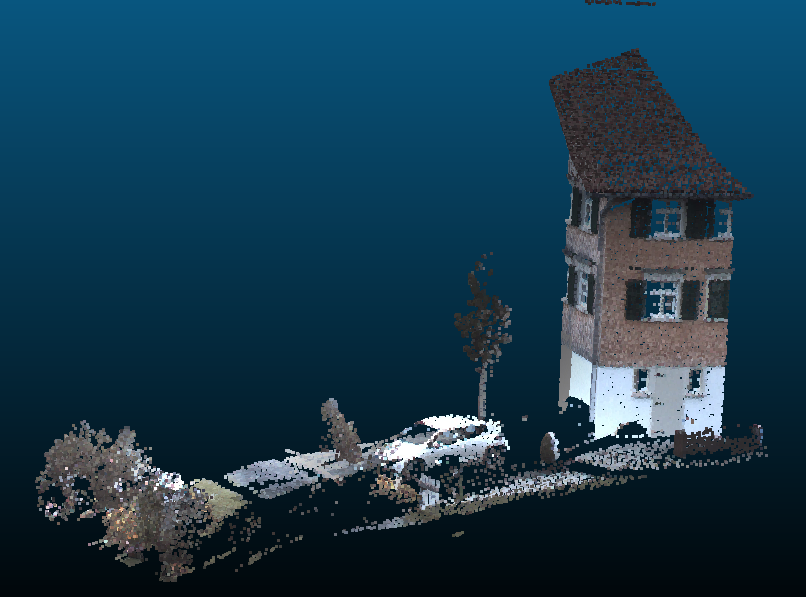
\includegraphics[width=0.8\textwidth]{fig/smallcloud_0.png}
    \caption{Petit nuage de points utilisé pour les tests}
    \label{fig:smallcloud}
\end{figure}

\subsubsection*{Premier algorithme}
Les voxels choisis par les auteurs sont parallélépipédiques rectangles (en anglais \emph{cuboids}). On commence par définir $s_\text{max}$ la taille maximale d'un voxel (dans chacune des trois dimensions de l'espace). La méthode proposée par les auteurs repose sur l'heuristique suivante :
\begin{enumerate}
	\item On commence par construire un \emph{arbre kd} des coordonnées du nuage de points ;
	\item On sélectionne un point au hasard dans le nuage et on détermine son $\frac{s_{\text{max}}}{2}$-voisinage grâce à l'\emph{arbre kd}. On appelle $\mathcal{W}$ l'ensemble des points de ce voisinage qui n'ont pas déjà été inclus dans un voxel ;
	\item On détermine la plus petite boîte parallélépipédique $\mathcal{B}$ englobant les points de $\mathcal{W}$ ;
	\item On définit un nouveau voxel $\V$ en sélectionnant tous les points du nuage qui sont contenus dans $\mathcal{B}$ et qui n'ont pas encore été inclus dans un autre voxel.
	\item On retourne au point 2 jusqu'à ce qu'il n'y ait plus de points à sélectionner.
\end{enumerate}

Cet algorithme converge nécessairement car le nombre de points qui restent sélectionnables décroît strictement à chaque itération (au moins un point est mis dans un voxel à chaque fois, celui sélectionné à l'étape 2). Malgré son efficacité, cet algorithme a cependant l'inconvénient de sélectionner les centres des voxels au hasard : il est possible qu'il décide de prendre un point se trouvant juste à côté de deux voxels déjà sélectionnés, ce qui amènera à des voxels de taille très diverses. 

\subsubsection*{Version alternative}
Pour pallier cet inconvénient, nous proposons une deuxième méthode alternative pour rééquilibrer les tailles des voxels : au lieu de sélectionner les points centraux au hasard, on échantillonne l'espace selon une grille régulière.

\begin{enumerate}
\item On construit un \emph{arbre kd} des coordonnées du nuage de points
\item On échantillonne l'espace selon une grille dont les mailles sont de taille $s_\text{max} \times s_\text{max}\times s_\text{max}$ et on ne garde que les points de cette grille qui sont à une distance inférieure à $\sqrt{3}\ s_\text{max}$ d'au moins un point du nuage en utilisant l'\emph{arbre kd} défini précédemment. On note $\mathcal{C}$ les points de cette grille restants après cette étape et on construit un nouvel \emph{arbre kd} sur $\mathcal{C}$.
\item On associe chaque point du nuage à l'élément de $\mathcal{C}$ le plus proche en effectuant une recherche du plus proche voisin grâce l'\emph{arbre kd} sur $\mathcal{C}$.
\end{enumerate}

La figure \ref{fig:voxelcloud} compare les nuages de voxels obtenus après application des deux méthodes. On y a affiché uniquement les centres géométriques des voxels, qui ont évidemment plus de structure sur la figure de droite. Cette structure ajoute certes un petit biais dû à la grille sous-jacente sélectionnée mais elle a l'avantage de diminuer le nombre de voxels trop petits et de plus remplir les voxels en moyenne. Nous avons pour ces raisons préféré cette méthode. 

\begin{figure}[h]
    \centering
    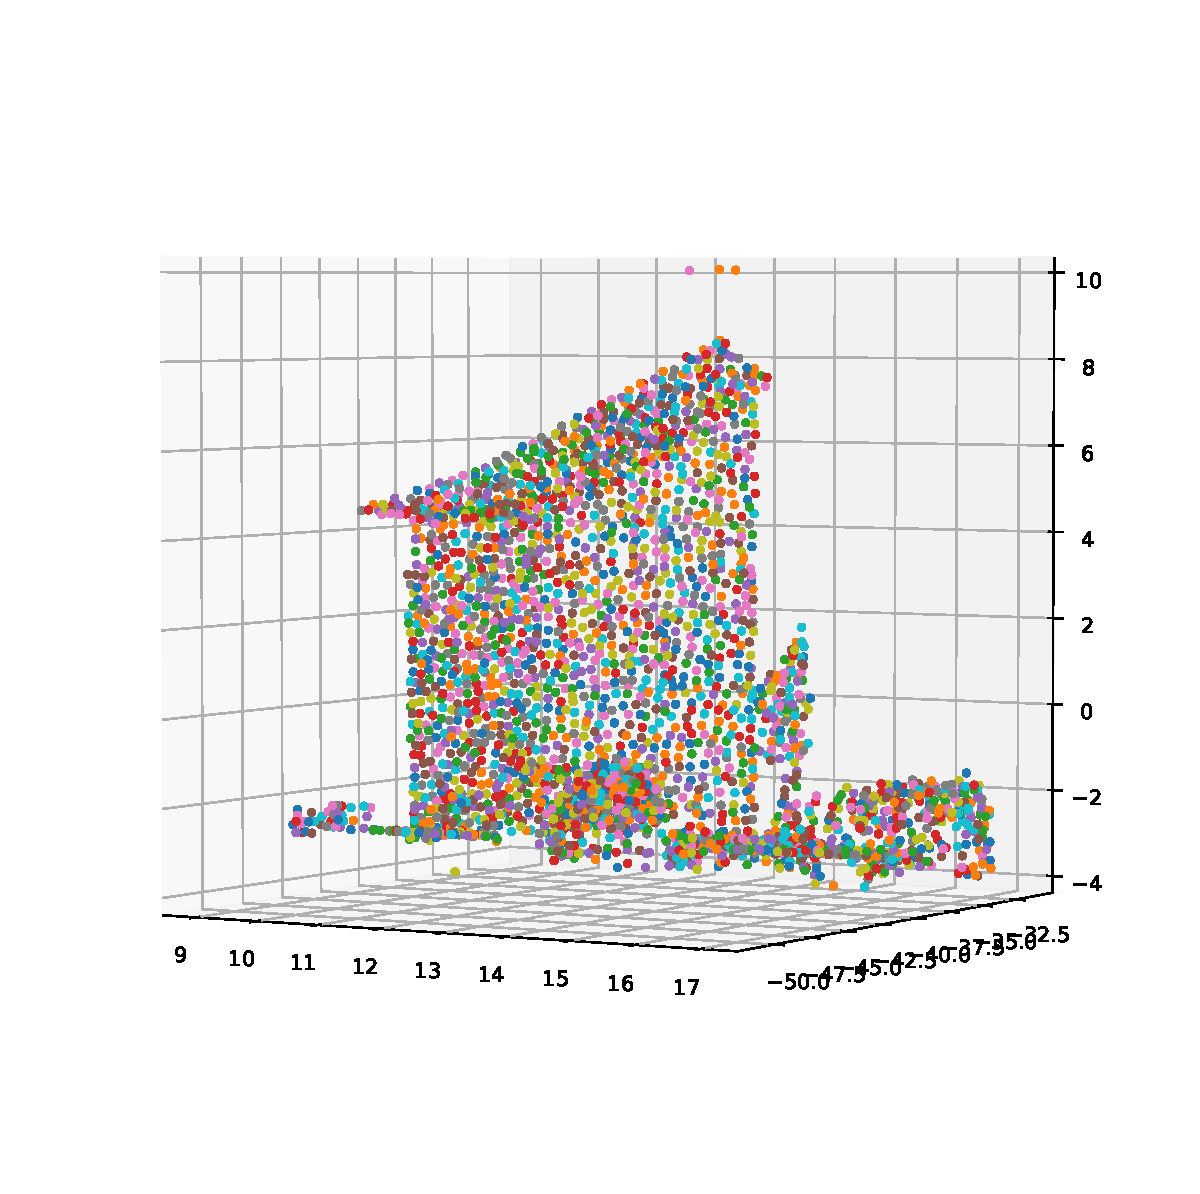
\includegraphics[width=0.5\textwidth]{fig/figgridnonregular.pdf}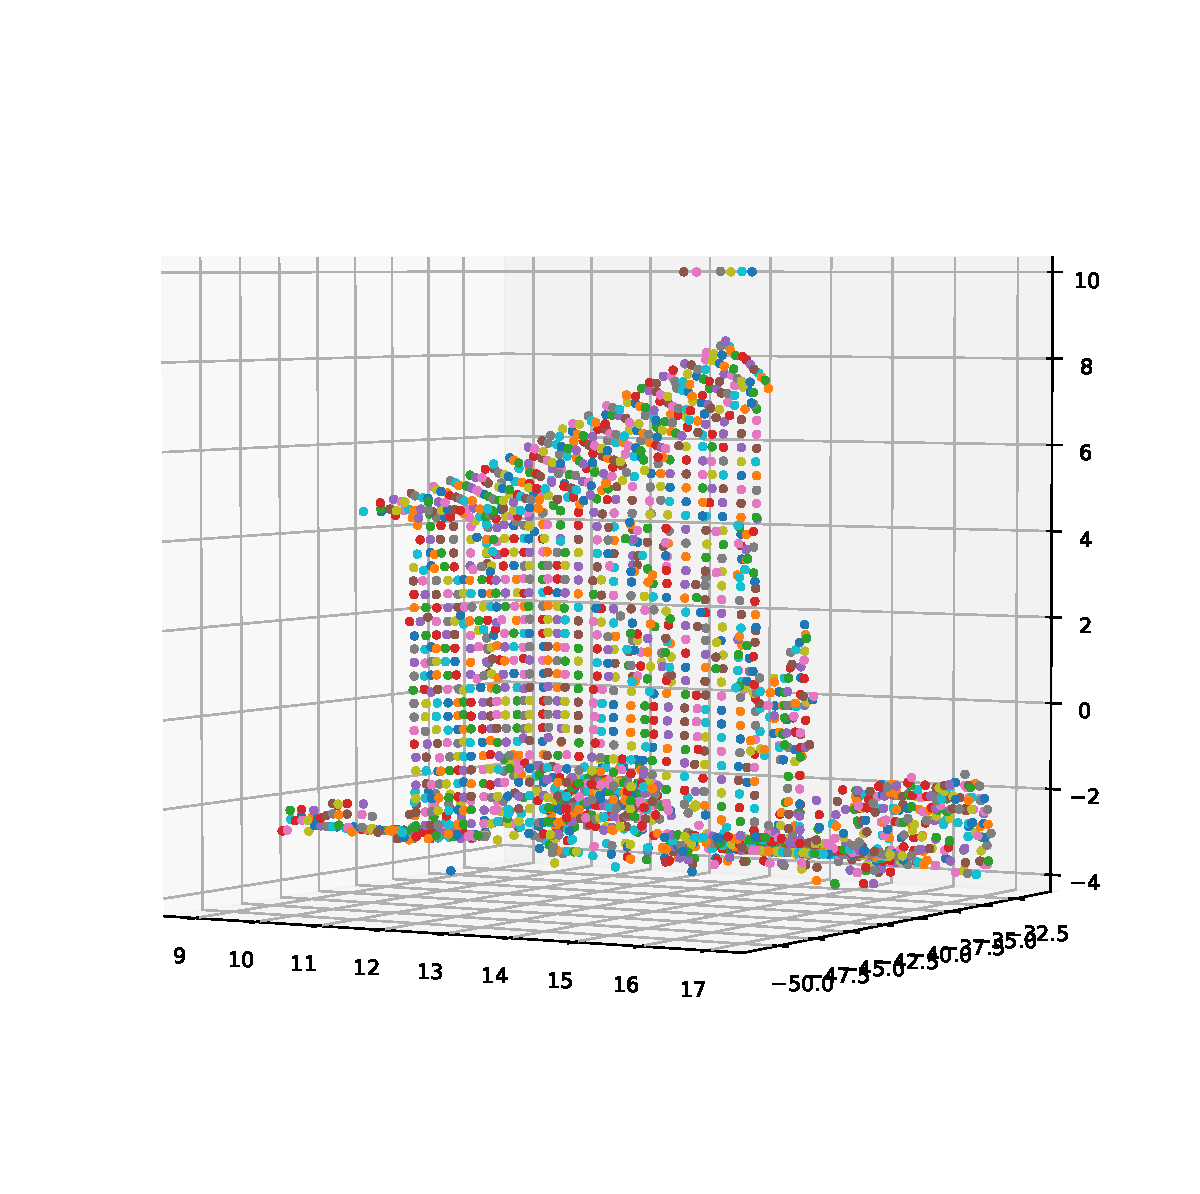
\includegraphics[width=0.5\textwidth]{fig/figgridregular.pdf}
    \caption{Nuages de voxels obtenus à l'aide de l'algorithme directement issu de l'article (points tirés de façon aléatoire) [figure de gauche] et à l'aide de l'algorithme alternatif (points tirés selon une grille régulière) [figure de droite]. Chaque voxel est représenté avec une couleur aléatoire.}
    \label{fig:voxelcloud}
\end{figure}

\subsubsection*{Post-traitement des voxels}
Certains voxels obtenus après cette étape seront de taille trop petite pour être significative : il est par exemple impossible de définir une normale au voxel si celui-ci ne contient qu'un ou deux points. On décide donc de supprimer les voxels trop petits : si $A$ est un voxel possédant moins de $\kappa \geq 3$ points, on associe ses points constitutifs au voxel $B$ le plus proche si la taille de $B$ le permet (par exemple si $B$ est un voxel d'un lampadaire, il aura une étendue très faible dans les directions $\overrightarrow{x}$ et $\overrightarrow{y}$ et on lui associera plus volontiers des points en-dessous ou au-dessus de lui que des points autour de lui dans le plan $(\overrightarrow{x},\overrightarrow{y})$. On met enfin de côté les points qu'on est incapable d'associer à un voxel suffisamment gros : la figure \ref{fig:non-associes} présente le nuage de voxels après cette étape : les croix noires représentes les points 3D qui n'ont pas été retenus dans le nuage de voxels.

Cette étape est effectuée dans la fonction \texttt{postprocess\_small\_voxels} de chaque objet \texttt{VoxelCloud}.

\begin{figure}[h]
    \centering
    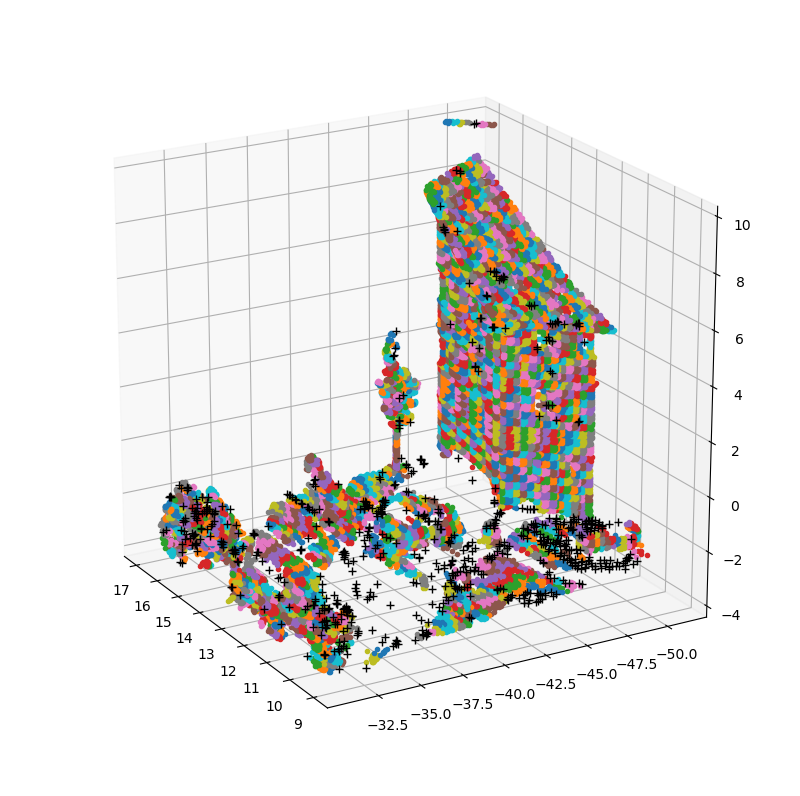
\includegraphics[width=0.6\textwidth]{fig/with_unassociated_points.png}
    \caption{Nuage de voxels post-traité : les croix noires correspondent aux points du nuage de points initial qui n'ont pas été considérés dans un des voxels car trop isolés. Dans ca cas particulier, cela correspond à $1.8\%$ des points.}
    \label{fig:non-associes}
\end{figure}

\subsection{Calcul des caractéristiques des voxels}
\label{partie-caracteristiques-voxels}
Une fois les points composant chaque voxel déterminés, il est possible de calculer les caractéristiques locales en associant à chaque voxel $\V$:

\begin{itemize}
\item son centre géométrique $\overrightarrow{p_\V}$ (que l'on suppose être le point au milieu de la boîte parallélépipédique définie au point 3 de la la partie \ref{partie-algo-voxels}) et sa taille $\overrightarrow{s_\V}$ (taille de la boîte $\mathcal{B}$ dans les 3 dimensions spatiales);
\item sa couleur, définie par la moyenne $\overrightarrow{\mu_\V^c}$ et l'écart-type $\overrightarrow{\sigma_\V^c}$ locaux de chaque canal de la couleur RVB des points constitutifs de $\mathcal{V}$ ;
\item son intensité de réflectance laser, définie par la moyenne $\mu_\V^i$ et l'écart-type $\sigma_\V^i$ locaux de l'intensité de réflectance laser des points constitutifs de $\mathcal{V}$ ;
\item son vecteur normal $\overrightarrow{n_\V}$, déterminé par analyse des composantes principales de tous les points constitutifs de $\mathcal{V}$
\end{itemize}

On a noté avec des flèches $\overrightarrow{\cdot}$ les quantités vectorielles, sur lesquelles on sera amené par la suite à effectuer des opérations (comparaison, somme, ...) terme à terme.

Il est bien entendu également possible de calculer d'autres caractéristiques comme la planarité ou la linéarité de chaque voxel. Ces caractéristiques pourront par exemple être utilisées ultérieurement lors de la classification.

Ces calculs sont effectués dans la fonction \texttt{compute\_features} de chaque objet \texttt{VoxelCloud}.

\section{Voisinage dans l'espace des voxels et segmentation}
L'étape suivante proposée dans \cite{aka_article} est la segmentation des voxels pour en déduire des objets qui pourront ensuite être classifiés. On propose dans cette partie une nouvelle lecture de la méthode \emph{link-chain} proposée dans l'article en l'interprétant comme la détection de composantes connexes dans un graphe dont les arêtes sont définies par une nouvelle relation de voisinage mélangeant informations spatiale et colorimétrique. 


\subsection{Condition de voisinage}
\label{condvoisinage}
On se place dans l'ensemble $\mathcal{Z} = \{\mathcal{V}\}$ des voxels que l'on munit d'une relation de voisinage grâce aux caractéristiques des voxels calculées précédemment.

Soit $A, B \in \mathcal{Z}$ deux voxels et $c_D > 0$. On dit que $A$ et $B$ sont $c_D$-voisins, et on note $A \sim_{c_D} B$ si :

\begin{align}
\left|\overrightarrow{p_A} - \overrightarrow{p_B}\right| &\leq c_D\overrightarrow{1} + \frac{1}{2} \left(\overrightarrow{s_A} + \overrightarrow{s_B}\right)\label{cond1}\\
\left|\overrightarrow{\mu_A^c} - \overrightarrow{\mu_B^c}\right| &\leq 3 \max\left(\overrightarrow{\sigma_A^c}, \overrightarrow{\sigma_B^c}\right)\label{cond2}\\
\left|\mu_A^i - \mu_B^i\right| &\leq 3 \max\left(\sigma_A^i, \sigma_B^i\right)\label{cond3}
\end{align}

On remarque immédiatement que cette relation est symétrique : $A \sim_{c_D} B \Leftrightarrow B \sim_{c_D} A$. On peut alors en munir notre ensemble $\mathcal{Z}$ d'arêtes pour former un graphe non-orienté dont on détermine ensuite les composantes connexes.

\paragraph*{Interprétation des conditions}
\begin{itemize}
\item Condition (\ref{cond1}) : les centres des deux voxels doivent être séparés d'au plus la moyenne des tailles des deux voxels, plus un facteur correctif $c_D$ permettant d'élargir la taille des voisinages (par exemple en cas de de nuage peu dense). Ainsi, à distance inter-centre constante, $A$ et $B$ seront voisins s'ils sont suffisamment gros. S'ils sont peu étendus dans la direction de la droite reliant les centres, on retiendra l'hypothèse qu'ils ne sont pas voisins.
\item Condition (\ref{cond2}) : la différence de couleur doit être inférieure à trois fois le plus grand écart-type. Ainsi, si une zone a une forte variabilité colorimétrique (écart-type grand), la condition sera plus permissive que si les points sont tous strictement de la même couleur.
\item Condition (\ref{cond3}) : elle s'interprète exactement comme la condition (\ref{cond2}) mais avec les intensités de réflectance laser.
\end{itemize}

\subsection{Recherche des composantes connexes}
La recherche des composantes connexes pourrait se faire de façon naïve en $\mathcal{O}(|\mathcal{Z}|^2)$ en parcourant l'ensemble $\mathcal{Z}$ pour chaque voxel et en vérifiant la condition de voisinage pour chaque paire de points. Toutefois, on peut considérablement alléger les calculs en restreignant la vérification de la condition aux voxels spatialement proches et en utilisant pour ceci un \emph{arbre kd}. Il suffit alors d'effectuer un parcours en profondeur du graphe défini par la relation de voisinage du paragraphe précédent. Les détails de la méthode sont présentés dans la fonction \texttt{compute\_connected\_components} de la classe \texttt{VoxelCloud}. Celle-ci se base sur trois fonctions avant d'effectuer un parcours en profondeur :
\begin{itemize}
    \item \texttt{are\_neighbours(i,j)} qui vérifie si deux voxels sont voisins (en $\mathcal{O}(1)$)
    \item \texttt{find\_spatial\_neighbours(i)} qui renvoie les voisins géométriques du voxel \texttt{i}, qui ont donc une chance d'être voisins, il y en a généralement un nombre fini $\ll |\mathcal{Z}|$
    \item \texttt{find\_neighbours(i)} qui retourne tous les voisins d'un voxel en s'appuyant sur les deux fonctions précédentes
\end{itemize}

\subsection{Segmentation du sol}
\label{segmentation-sol}
Les composantes connexes obtenues par la méthode précédente ne sont pas immédiatement satisfaisantes car encore trop peu segmentées, comme on peut le voir sur l'image de gauche de la figure \ref{fig:first_segmentations} où l'on a affiché en couleurs les différentes composantes connexes obtenues avec $c_D = 0.25\text{m}$ et $s_\text{max}=0.3\text{m}$. Le sol a tendance à agir comme un pont entre les objets et la modification des conditions de voisinage (par exemple en jouant sur le paramètre $c_D$) a pour effet soit de sur-segmenter certaines zones soit d'en sous-segmenter d'autres. Dans le cas étudié sur cette image, on voit notamment que l'arbre, la voiture et le sol entre les deux ont été regroupés dans une même composante connexe. 

L'article propose cependant une méthode permettant de régler ce problème : il inclut une information \emph{a priori} sur le nuage de points : celle que la scène étudiée comporte un sol relativement plat et étendu. Parvenir à éliminer le sol permet alors de segmenter correctement les objets restants avant de les classifier.
La méthode employée par les auteurs pour segmenter le sol repose sur un seuillage de la valeur de l'orientation des normales avec l'axe vertical (voir page 1632). Cette méthode ne nous a pas paru totalement satisfaisante car nos jeux de données pouvaient avoir des pentes importantes. Nous avons donc choisi à la place d'utiliser l'algorithme RANSAC \cite{ransac} et de l'utiliser pour détecter et retirer le plus grand plan de la scène (que l'on suppose être le sol). Nous avons un peu affiné l'algorithme pour le faire fonctionner sur des voxels et non des points, ainsi qu'en ajoutant une condition sur l'orientation du plan trouvé qui ne doit pas trop s'éloigner de l'horizontale afin d'éviter de trouver un grand mur étendu dans une rue par exemple). Les détails d'implémentation peuvent être analysés dans le fichier \texttt{ransac.py} et le résultat est présenté à droite de la figure \ref{fig:first_segmentations} : cette fois-ci, l'arbre et la voiture, ont notamment été segmentés correctement, tout comme le morceau de sol proche de la maison.

\begin{figure}[h]
    \centering
    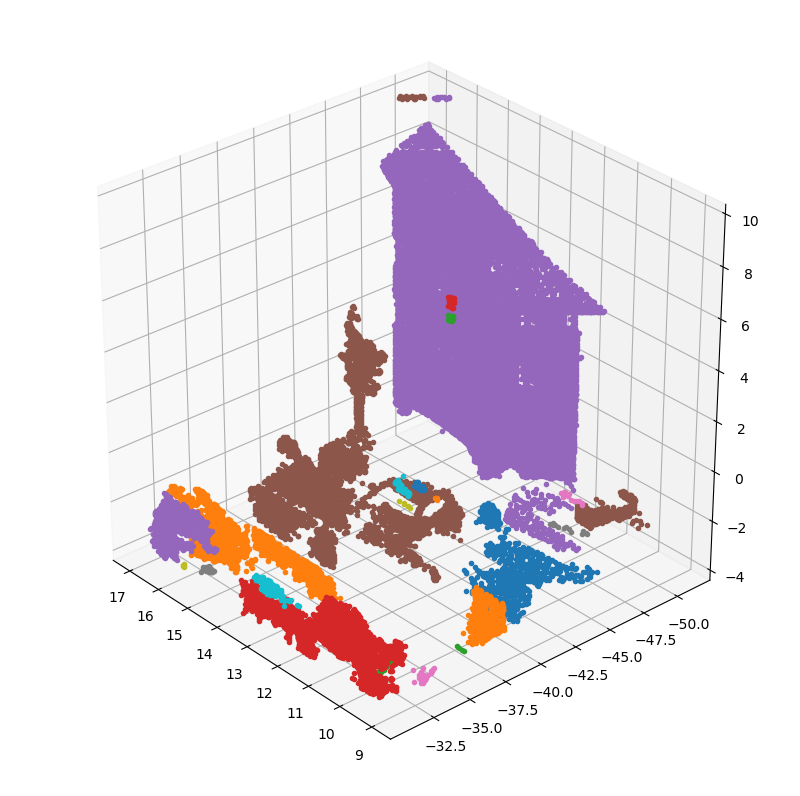
\includegraphics[width=0.5\textwidth]{fig/first_segmentation.png}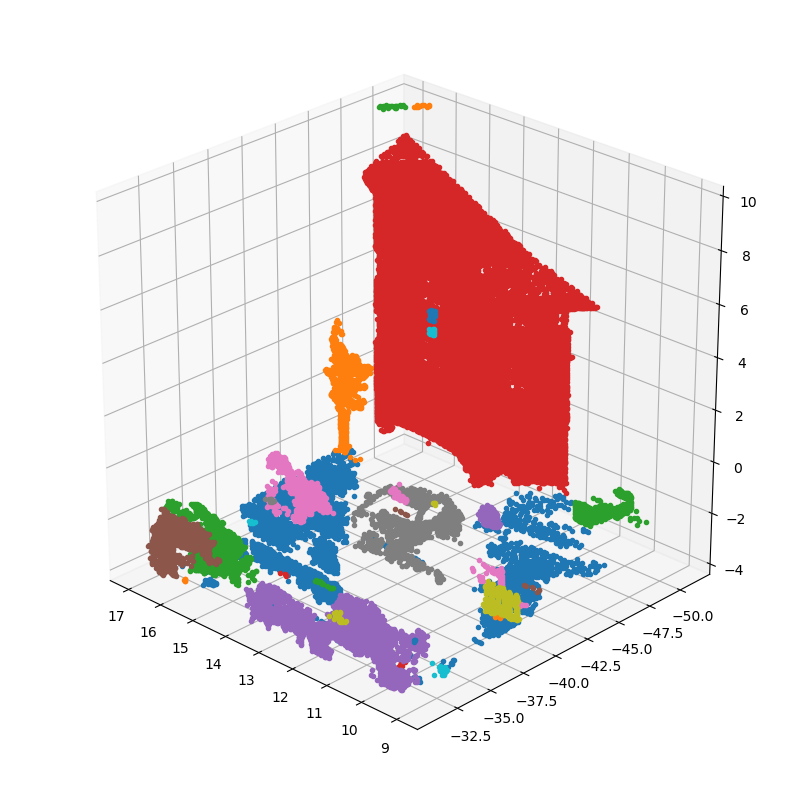
\includegraphics[width=0.5\textwidth]{fig/second_segmentation.png}
    \caption{Segmentations obtenues sur le nuage de test avant [gauche] et après [droite] avoir retiré le sol grâce à l'algorithme RANSAC (condition de coplanarité : 20cm)}
    \label{fig:first_segmentations}
\end{figure}

\subsection{Méthodes alternatives de recherche des composantes connexes}
La méthode proposée par les auteurs et que nous avons présentée jusqu'ici se place dans un contexte extérieur, suppose que le sol est relativement plat et que les objets peuvent être séparés aisément dès que le sol est retiré du nuage de voxels. Nous nous sommes cependant posé la question de l'efficacité de la méthode dans d'autres contextes : il est probable que la présence de nombreux objets entremêlés ou un sol irrégulier puissent considérablement détériorer les performances de la segmentation, qui est pourtant une étape cruciale avant de pouvoir effectuer la classification (une segmentation mal faite mènera forcément à de mauvais résultats car on essaiera de classifier des objets entremêlés ou alors des morceaux d'objets). Nous avons donc réfléchi à deux méthodes alternatives : l'une non supervisée basée sur le partitionnement spectral du graphe d'adjacence et l'autre supervisée basée sur l'apprentissage de la relation de voisinage entre voxels.

\subsubsection{Partitionnement spectral}
Les auteurs de \cite{aka_article} mentionnent dans leur revue de littérature la possibilité d'effectuer un partitionnement de graphe, en citant notamment l'article \cite{mincut}. Nous avons repris l'idée en étendant la matrice d'adjacence définie par la condition de voisinage du paragraphe \ref{condvoisinage} pour avoir des entrées moins brutales qu'une simple matrice binaire indiquant si les points sont voisins ou non. On construit à la place une matrice de similarité indiquant le degré de proximité des voxels du nuage (fonction \texttt{similarity(i,j)} de la classe \texttt{VoxelCloud}).

Comme expliqué dans \cite{kernels} (pp. 168-181, 475-486, 506), si l'on définit le laplacien du graphe comme étant la différence de la matrice des degrés et de la matrice d'adjacence (la matrice de similarité définie précédemment)

$$L\hat{=}D-A$$

Alors le pseudo-inverse de $K$ de $L$ définit un noyau reproduisant sur l'espace de Hilbert 
$$\mathcal{H}~=~\left\{f:\mathcal{Z}\rightarrow \R \middle/ \sum_{z\in\mathcal{Z}}f(z)=0\right\}$$ de fonctions valeur du graphe sommant à 0 (on rappelle qu'on note $\mathcal{Z}$ l'ensemble des nœuds du graphe, ie. les voxels).

On peut alors partitionner le graphe en cherchant une fonction $f\in\mathcal{H}$ qui minimise $f^TLf$, par exemple sous la contrainte $\sum_{z\in\mathcal{Z}}f(z)^2=0$, ce qui revient à effectuer une analyse des composantes principales non-linéaire avec le noyau $K$. Les directions les plus significatives seront données par les vecteurs propres associés aux plus grandes valeurs propres de $K$, donc les plus petites valeurs propres de $L$. Il suffit donc de diagonaliser le laplacien $L$ et d'en extraire les $k$ plus petites valeurs propres et surtout les vecteurs propres associés, qui sont des fonctions de graphe (des applications qui associent un nombre réel à chaque voxel). On peut ensuite effectuer un partitionnement non-supervisé (par exemple avec l'algorithme \emph{k-moyennes} ou bien un mélange de gaussiennes) dans l'espace à $k$ dimensions et $|\mathcal{Z}|$ individus défini par les $k$ fonctions valeurs retenues pour déduire un partitionnement du graphe. L'implémentation encore très expérimentale peut être explorée dans la fonction \texttt{find\_connected\_components\_similarity} de la classe \texttt{VoxelCloud}.

On peut voir à la figure \ref{fig:network_kernel} le graphe d'adjacence pondéré par la matrice de similarité, affiché avec la bibliothèque \texttt{networkx}. Des points proches ont une forte similarité, des points éloignés ont une faible similarité. L'idée est d'essayer de trouver la bonne matrice de similarité pour que les objets soient le plus séparés possible dans le graphe, afin que l'algorithme de partitionnement spectral arrive à couper lui-même au bon endroit. La figure \ref{fig:resultat-segmentation-spectrale} montre le résultat de la méthode appliquée au jeu de données de test habituel : l'algorithme arrive de lui-même à séparer la voiture et l'arbre du sol, et même la route (en vert) des autres types de sol.

\begin{figure}[h]
    \centering
    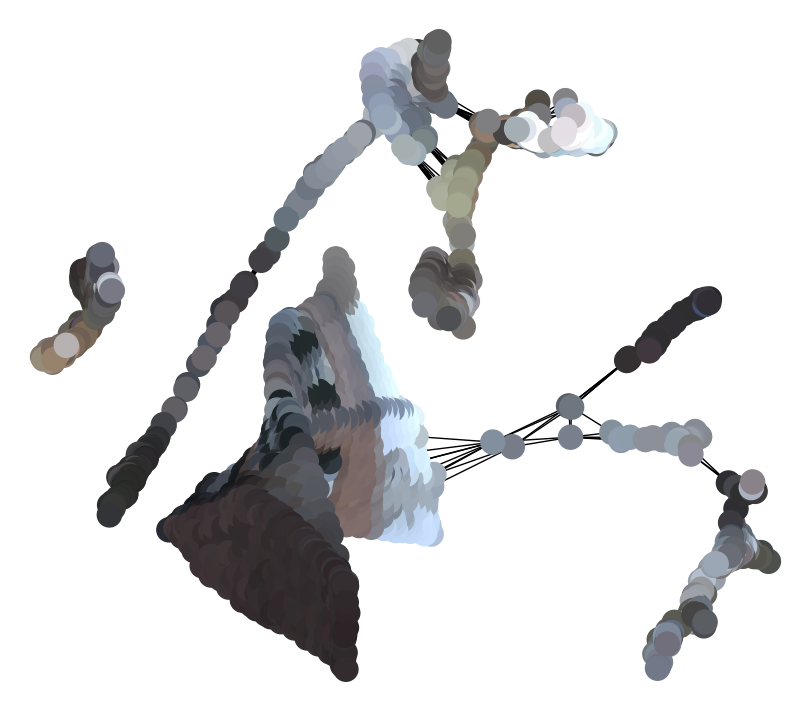
\includegraphics[width=0.5\textwidth]{fig/nx_graph.png}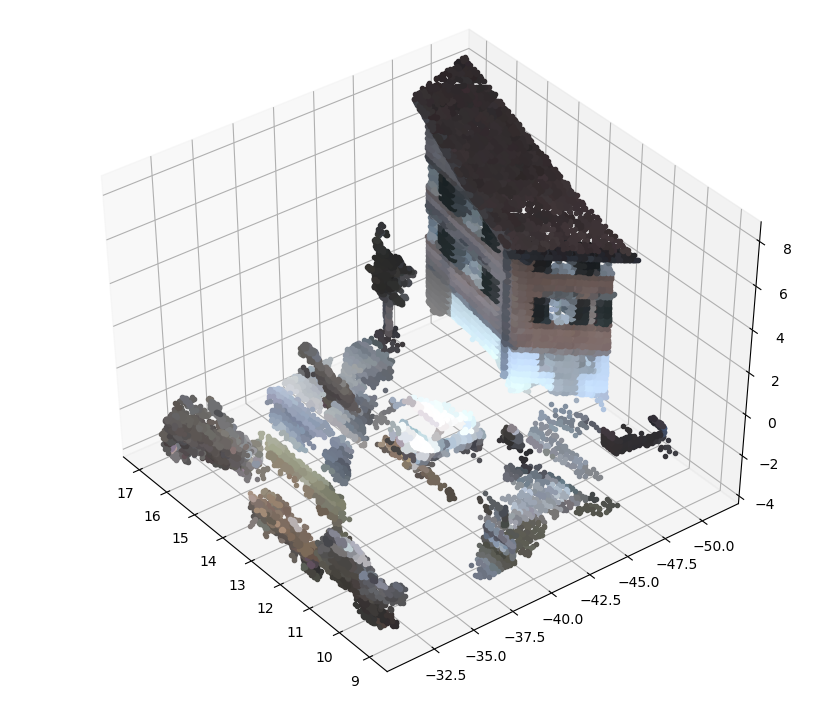
\includegraphics[width=0.5\textwidth]{fig/nx_3d_realcolor.png}
    \caption{Graphe défini par la relation de similarité sur l'exemple de test, affiché en vraies couleurs et scène 3D correspondante. On reconnaît que les gros clusters sont des objets de la scène que l'on aimerait en effet segmenter ensemble, comme la maison, le bac à droite de la porte (en noir) ou la voiture (l'excroissance blanc-beige en haut à droite du graphe). L'idée de la méthode est d'améliorer la relation de similarité pour que les objets se séparent d'eux-mêmes sur le graphe avant d'appliquer une méthode de partitionnement de graphe.}
    \label{fig:network_kernel}
\end{figure}

\begin{figure}[h]
    \centering
    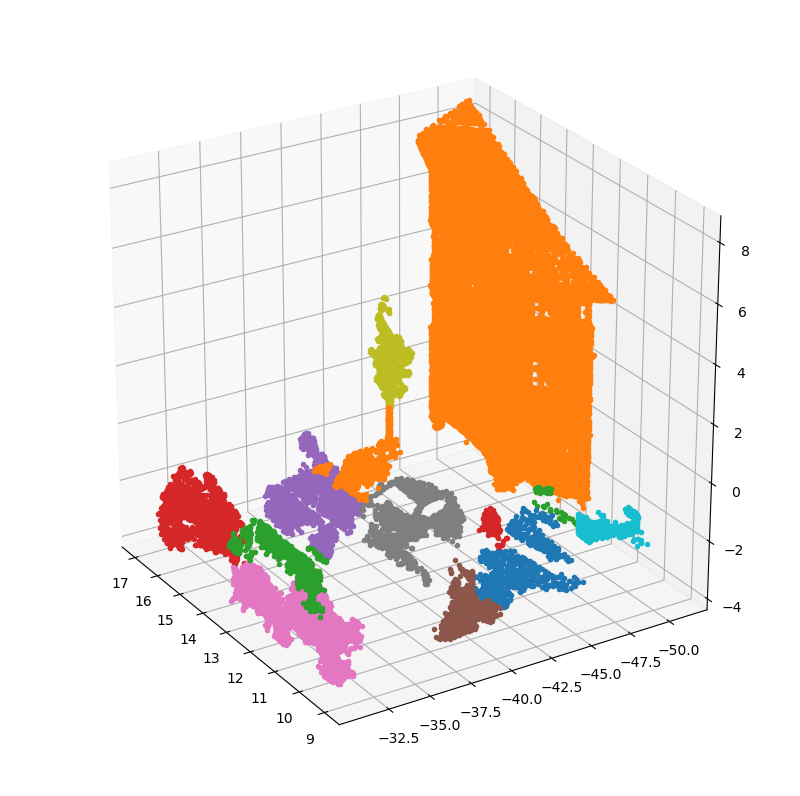
\includegraphics[width=0.6\textwidth]{fig/third_segmentation_spectral.png}
    \caption{Résultat de la méthode de segmentation spectrale en prenant $k = 14$ composantes dans l'algorithme $k$-moyennes.}
    \label{fig:resultat-segmentation-spectrale}
\end{figure}

Les résultats très encourageants de cette méthode pour ce cas particulier sont à nuancer par plusieurs inconvénients. Elle est beaucoup aidée par la connaissance \emph{a priori} du nombre d'objets à segmenter, elle est très coûteuse en calculs (avec notamment une diagonalisation d'une matrice ayant la même taille que le nombre de voxels) et elle nécessite de trouver une fonction de similarité suffisamment satisfaisante pour le problème considéré. Des solutions sont envisageables pour chacun de ces problèmes, mais leur étude nécessitera du temps. On pourra se référer pour une étude plus approfondie du partitionnement spectral à \cite{spectralclustering}.

\subsubsection{Apprentissage supervisé}
Une méthode alternative que nous avons essayée est d'apprendre de manière supervisée la relation de voisinage entre voxels. L'objectif était d'avoir une condition d'association de voxels voisins plus robuste que celle proposée dans \cite{aka_article} en reposant sur un plus grand nombre de paramètres et en adaptant les critères de décision à la nature du nuage de points (il n'existe pas a priori une méthode de segmentation qui fonctionnerait pour tout type de nuage de points). La méthode proposée cherche, à partir d'un vecteur de paramètres qui qualifient une paire de voxels (delta des couleurs, de la réflectance laser, du centre géométrique ou encore de la planarité, verticalité, sphéricité, linéarité...), à déterminer si deux voxels sont voisins. 

Dans cette étude, pour la phase d'apprentissage, nous considérons que deux voxels sont réellement voisins si d'une part ils sont assez proches et d'autre part s'ils partagent le même label avec un seuil de pureté acceptable (i.e.\ le label dominant doit être partagé par au moins un certain pourcentage des pixels à l'intérieur du voxel). Il faut alors entrainer un classifieur binaire. 

Notons maintenant que considérer l'ensemble des paires de voxels possibles n'est pas très judicieux car la notion de voisinage n'a un sens que si les voxels sont proches. Pour restreindre le nombre de paires, nous avons donc choisi de préfiltrer les paires en appliquant la condition sur les distances mentionnée dans  \cite{aka_article}. De plus, comme notre méthode de segmentation s'appuie sur le filtrage du sol, il n'y a pas d'intérêt à apprendre ce qu'est la relation de voisinage pour les voxels du sol (d'autant plus que ceux-ci sont en grand nombre et pourraient polluer l'apprentissage). Nous faisons donc le choix de filtrer les voxels du sol avant de sélectionner les paires. 

Une dernière difficulté : les composantes connexes étant assez denses, des voxels proches sont souvent voisins (dans le sens défini ci-dessus).  Il y a donc a priori un grand déséquilibre dans les données d'entrainement entre les deux classes (voisin / non-voisin). Ceci peut être néfaste pour l'entraînement, nous avons donc procédé à un rééquilibrage des classes (voisin / non-voisin) en amont de l'apprentissage. 

Nous avons enfin choisi comme classifieur un \emph{Random Forest} (forêt d'arbres décisionnels) composée de $20$ arbres de décision. Une fois le classifieur de voisinage appris, nous pouvons appliquer cette relation de voisinage à de nouveaux nuages de points et ainsi déterminer les composantes connexes de ces nuages.

La figure \ref{fig:resultat-segmentation-supervisee} montre le résultat de cette méthode appliquée à la segmentation de la même scène que précédemment. On parvient à bien identifier la maison, l'arbre ainsi que le sol. Les objets au dessus du sol forment des amas unis. En prenant un seuil de tolérance trop permissif lors de la détection du sol, le toit de la voiture est souvent assimilé à du sol, cela a été réglé en optimisant ce seuil. Cependant, dans le cas présent, la voiture est détectée en plusieurs morceaux, ce qui ne facilitera pas sa classification.

\begin{figure}[h]
    \centering
    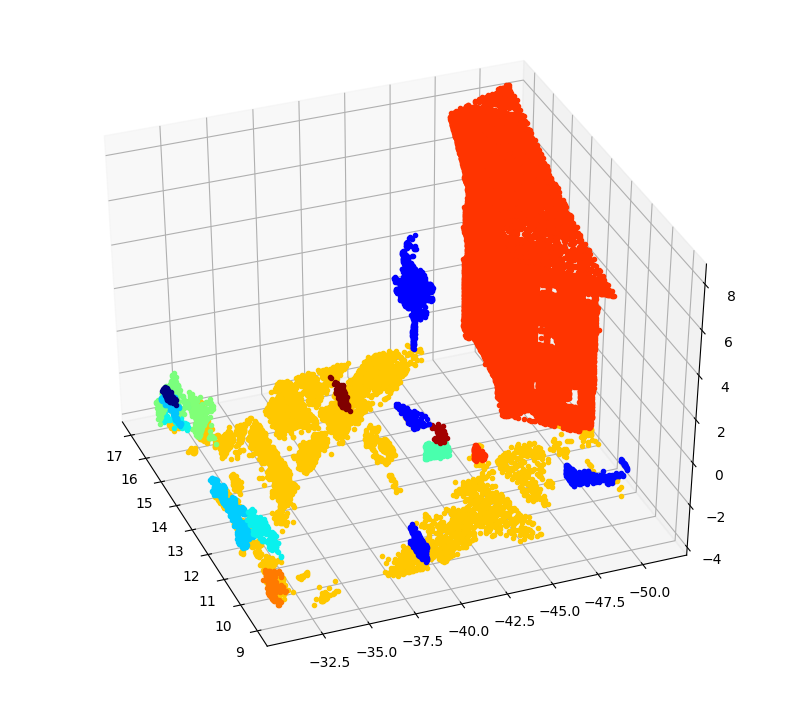
\includegraphics[width=0.6\textwidth]{fig/fourth_segmentation_supervised.png}
    \caption{Résultat de la méthode de segmentation par apprentissage supervisé de la relation de voisinage (voir la suite pour prendre connaissance des nuages utilisés lors de l'entraînement).}
    \label{fig:resultat-segmentation-supervisee}
\end{figure}

Cette méthode a donné des résultats plutôt satisfaisants sur de grands nuages de points, c'est donc celle que nous avons retenue pour traiter le jeu de données Semantic3D mentionné plus bas.

\section{Classification des objets segmentés}
La dernière étape de la méthode est enfin la classification des composantes connexes du nuage de points. Nous présentons dans ce qui suit la méthode proposée par l'article, notre implémentation ainsi que la métrique utilisée.

\subsection{Méthode}
La méthode de classification introduite repose sur l'agrégation des caractéristiques des voxels des composantes connexes. Supposons que l'on veuille classifier un objet qui a été segmenté en une composante connexe : cet objet est constitué de plusieurs voxels, chacun ayant certaines caractéristiques qui ont été calculées à la partie \ref{partie-caracteristiques-voxels}. L'idée est alors simplement de regarder \og de loin \fg\ à quoi ressemble cet objet en observant une ou plusieurs fonctions de ces caractéristiques, des \emph{features}. Par exemple, on peut calculer la moyenne des couleurs des voxels composant l'objet et déterminer s'il s'agit plutôt d'herbe ou d'asphalte. Ou encore observer le barycentre de l'objet et le comparer à son centre géométrique.

Cependant, la méthode exacte de \cite{aka_article} est peu détaillée et repose sur de simples seuils arbitrairement choisis sur certaines fonctions des caractéristiques des voxels. Nous avons donc décidé d'appuyer notre méthode sur les mêmes paramètres (que nos avons d'ailleurs enrichis) et d'apprendre de manière supervisée la classification des composantes connexes. Pour reprendre les catégories de paramètres spécifiées dans \cite{aka_article}, nous avons considéré les paramètres liés :
\begin{itemize}
\item \textbf{aux normales} : la moyenne et la variance de la projection des normales des voxels de la composante connexe sur l'axe z ainsi que sur le plan défini par les axes x et y.
\item \textbf{au centre géométrique et au barycentre} : le centre géométrique de la composante connexe calculé à partir de l'ensemble des voxels de celle-ci, même chose pour le barycentre.
\item \textbf{à la couleur et l'intensité} : la moyenne et la variance des couleurs et de la réflectance laser des voxels de la composante connexe.
\item \textbf{à la forme géométrique} : les valeurs propres et vecteurs de la \emph{Principal Component Analysis} (PCA) des centres géométriques des voxels de la composante connexe, la moyenne de la verticalité, linéarité, planarité et sphéricité  des voxels de la composante connexe, le nombre de voxels dans la composante connexe et la taille de la composante connexe.
\end{itemize}
La taille des données s'y prêtant bien, nous avons choisi comme classifieur un \emph{Random Forest} (forêt d'arbres décisionnels) composée de $20$ arbres de décision. Il suffit alors d'utiliser les étiquettes \emph{labels} fournis dans le jeu de données et d'apprendre à classifier les objets en fonction de leurs \emph{features}.

\subsection{Métrique}

Afin dévaluer la pertinence de la classification nous proposons plusieurs métriques.

Tout d'abord des calculs de précision :
\begin{itemize}
\item \textbf{au niveau des composantes connexes} On attribue à l'ensemble des points de chaque composante connexe un unique label par vote de majorité sur les voxels qui la constituent. En effet, la segmentation n'étant pas toujours parfaite il se peut que des voxels de différents labels se retrouvent segmentés dans un même objet. On compare ensuite ce label de vérité terrain (obtenu par vote) au label prédit par le classifieur en chacun des points. Cette métrique permet de comparer la classification prédite à la meilleure classification possible en vue de la segmentation obtenue. Ainsi on peut évaluer la classification en se soustrayant des problèmes introduits par une mauvaise segmentation.

\item \textbf{au niveau des points} On peut également calculer la précision au niveau des points. Par ceci, on entend que la vérité terrain est donnée en chacun des points (et non plus pour chaque composante). Dans notre méthode, certains points ont été mis de côté parce qu'ils appartenaient à un voxel trop petit ou un voxel qui lui-même appartenait à un objet trop petit. Afin d'être plus juste, lors de la prédiction on attribue à ces points le label prédit du voxel le plus proche parmi les voxels qui appartiennent à des composantes connexes. Cette métrique rend compte de la qualité de la classification tout comme de la qualité de la segmentation.
\end{itemize}

Notons que l'article \cite{aka_article} propose une troisième voie, différente en évaluant l'erreur de classification au niveau des voxels. Ayant déjà deux métriques très complémentaires, nous n'avons pas jugé utile d'en utiliser une troisième dont les résultats devraient, en toute logique, se situer entre les résultats des deux métriques que nous venons de mentionner.

Quelle que soit la méthode choisie, on dispose d'une vérité terrain et d'une classification et on calcule alors la matrice de confusion qui donne le nombre (et on déduit aisément la proportion) de points bien et mal classifiés dans chaque classe.

\section{Données, résultats et conclusion}
\subsection{Implémentation}
L'implémentation de la méthode a été réalisée en Python. Elle est disponible à l'adresse suivante :

\begin{center}
	\url{https://github.com/h-sdl/projet-npm3d/} 
\end{center}

Cette implémentation reprend quelques éléments du code de Hugues Thomas\footnote{\url{mailto:huguesthomas218@gmail.com}} pour ce qui concerne le chargement et l'écriture de fichiers \texttt{.ply} représentant les nuages de points.

\subsection{Données}
\label{partie-donnees}
Les données mentionnées en 2013 dans l'article \cite{aka_article} n'étant plus disponibles en ligne en 2020, nous avons travaillé sur le jeu de données \texttt{semantic-8} de \href{http://www.semantic3d.net/}{\emph{Semantic3D}} \cite{hackel2017isprs}. Celles-ci ont l'avantage de comporter non seulement les données d'intensité de réflectance laser mais aussi de couleur RGB de chaque point, en plus d'être partiellement classifiées. Ce dernier point nous a permis de mettre en place une méthode de classification par apprentissage.
Nous avons d'abord réalisé nos expérimentations sur une version réduite du nuage \texttt{bildstein5} avant d'appliquer notre méthode à de plus gros nuages. Finalement nous avons sélectionné \texttt{domfountain1} et \texttt{untermaederbrunnen1} comme nuages d'entraînement, ainsi que \texttt{domfountain2}, \texttt{domfountain3}, \texttt{neugasse} et \texttt{untermaederbrunnen3} pour le test. Deux autres nuages \texttt{bildstein3} et \texttt{bildstein5}, plus difficiles, car comportant une colline ont aussi été utilisés pour tester davantage notre méthode. Les classes des différents objets fournis avec les nuages de points sont les suivantes : \texttt{terrain artificiel}, \texttt{terrain naturel}, \texttt{végétation haute}, \texttt{végétation basse}, \texttt{bâtiment}, \texttt{aménagement urbain}, \texttt{artefact de numérisation} et \texttt{voiture}. Nous n'avons gardé que les points annotés de ces nuages et avons fusionné les classes \texttt{terrain artificiel} et \texttt{terrain naturel} en \texttt{terrain} pour n'avoir qu'un seul type de sol, comme dans l'article que nous avons étudié.

Un extrait des données que nous avons utilisées est disponible à l'adresse suivante : 
\begin{center}
\url{https://cloud.mines-paristech.fr/index.php/s/ynK12DvoOrJ1LWA}
\end{center}
Tous les nuages ne sont pas disponibles mais ceux-ci permettront déjà au lecteur intéressé de mener ses premières expérimentations. Les données dans ce répertoire sont directement transformées à partir des données de \textit{Semantic3D} et sont disponibles sous licence CC BY-NC-SA 3.0.

\subsection{Résultats}

Les résultats globaux de la méthode la plus concluante sont visibles dans l'annexe \ref{annexe-resultats}, nuage par nuage. Nous avons choisi de comparer nos résultats à ceux de l'article \cite{aka_article} en utilisant les matrices de confusion qui permettent un examen plus précis de la répartition entre les différentes classes.

Nous présentons dans le reste de cette partie les résultats de certains points particuliers de notre implémentation des sous-méthodes et variantes détaillées dans les sections précédentes.

\subsubsection{Segmentation du sol}

Comme nous l'avons vu précédemment dans la partie \ref{segmentation-sol}, nous avons mis en place une méthode afin de segmenter le sol dans un premier temps. Ceci permet de faciliter la segmentation des autres objets, qui se retrouvent alors déconnectés des uns des autres pour la plupart. Nous comparons dans la Table \ref{table:ground} les résultats en terme de précision, toutes classes confondues, avec et sans cette méthode de segmentation du sol. On compare également les erreurs de classification classe par classe pour tous les nuages de l'ensemble de test dans la Figure \ref{fig:ground}.

\begin{figure}[p]
    \centering
    \subfloat[sans segmentation du sol]{{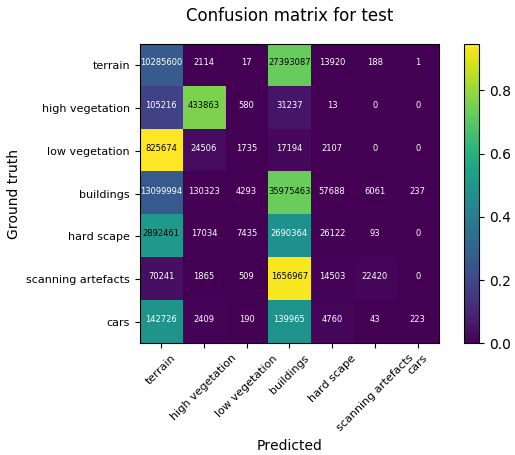
\includegraphics[width=8cm]{fig/test_without_ground_segmentation.png} }}
    \qquad
    \subfloat[avec segmentation du sol]{{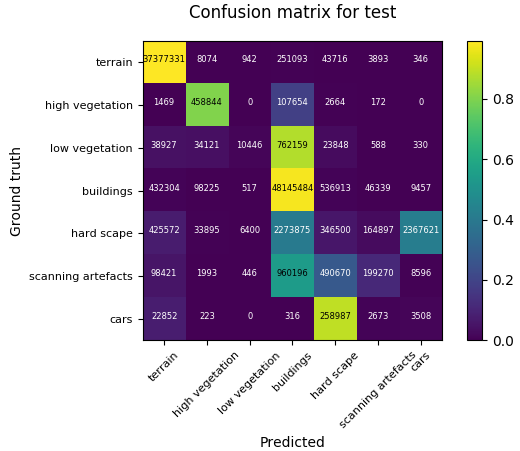
\includegraphics[width=8cm]{fig/test_with_ground_segmentation.png} }}
    \caption{Matrices de confusion pour le jeu de données de test, avec et sans segmentation du sol. On observe que sans segmentation du sol, en majorité trois classes sont détectées : le \texttt{terrain}, la \texttt{végétation haute} et les \texttt{bâtiments}. La \texttt{végétation basse} est confondue en grande partie avec le \texttt{terrain}. Les \texttt{voitures} et les \texttt{aménagements urbains} sont confondus entre le \texttt{terrain} et les \texttt{bâtiments}. Le \texttt{terrain} est quand à lui en grande partie assimilé aux \texttt{bâtiments}. Avec notre méthode de segmentation du sol, on voit une nette amélioration pour le \texttt{terrain}, d'une part celui-ci est bien mieux classifié, d'autre part beaucoup moins de classes sont confondues avec lui.}
    \label{fig:ground}
\end{figure}

% Test set precision metrics with and without ground segmentation
\begin{table}[p]
\caption{Précision (\%) au niveau des composantes connexes et des points, avec et sans segmentation du sol. On remarque une amélioration notable de la précision lorsque la vérité terrain est donnée au niveau des points. Cette amélioration est valable pour les données d'entraînement comme pour les données de test. Pour ce qui est de la précision lorsque la vérité terrain est donnée au niveau des composantes connexes, on remarques qu'avec notre méthode de segmentation du sol on obtient un score correct pour l'ensemble des nuages (entraînement et test), là où auparavant la classification pouvait être tout à fait fausse pour certains nuages du jeu de données de test (score proche de $0$\%).}

\begin{tabular}{l|c|c|c|c|}
\cline{2-5}
 & \multicolumn{4}{c|}{données d'entraînement} \\ 
\cline{2-5} 
 & \multicolumn{2}{c|}{domfountain1} & \multicolumn{2}{c|}{untermaederbrunnen1} \\
\cline{2-5} 
 & comp. & point & comp. & point \\
\hline
\multicolumn{1}{|l|}{sans segmentation du sol} & \textbf{100} & 56 & 99 & 51 \\
\hline
\multicolumn{1}{|l|}{avec segmentation du sol} & \textbf{100} & \textbf{92} & \textbf{100} & \textbf{93}\\
\hline
\end{tabular}

\bigskip

\begin{tabular}{l|c|c|c|c|c|c|c|c|}
\cline{2-9}
 & \multicolumn{8}{c|}{données de test}\\ 
\cline{2-9}
 & \multicolumn{2}{c|}{domfountain2} & \multicolumn{2}{c|}{domfountain3} & \multicolumn{2}{c|}{neugasse} & \multicolumn{2}{c|}{untermaederbrunnen3} \\ 
\cline{2-9}
& comp. & point & comp. & point & comp. & point & comp. & point\\
\hline
\multicolumn{1}{|l|}{sans segmentation du sol} & \textbf{99} & 57 & 2 & 46 & \textbf{99} & 52 & 2 & 38 \\
\hline
\multicolumn{1}{|l|}{avec segmentation du sol} & 94 & \textbf{92} & \textbf{95} & \textbf{94} & 97 & \textbf{91} & \textbf{90} & \textbf{85}\\
\hline
\end{tabular}
\label{table:ground}
\end{table}

\raggedbottom

\subsubsection{Apprentissage supervisée de la relation de voisinage}

Une autre amélioration que nous avons proposée est l'apprentissage supervisé de la relation de voisinage pour l'identification des composantes connexes (objets). Nous comparons les résultats obtenus avec le critère de voisinage de \cite{aka_article} appliqué tel quel et avec l'apprentissage de la relation de voisinage. Pour une comparaison juste, dans les deux cas on réalise au préalable la segmentation du sol à part. La précision pour les deux méthodes et pour les différents nuages est donnée dans la Table \ref{table:neighbourhood} et les résultats classe par classe sont donnés dans la Figure \ref{fig:neighbourhood}.

\begin{figure}[p]
    \centering
    \subfloat[critère de voisinage de \cite{aka_article}]{{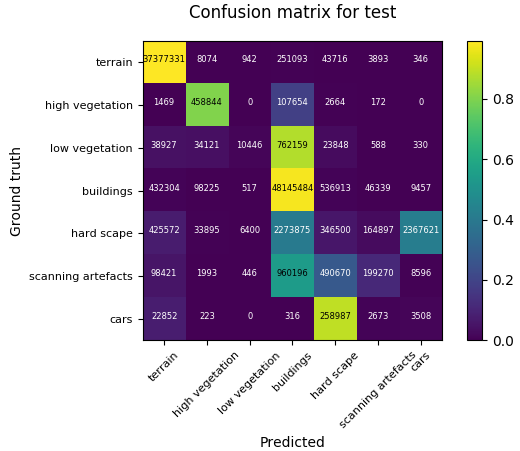
\includegraphics[width=8cm]{fig/test_with_ground_segmentation.png} }}
    \qquad
    \subfloat[apprentissage supervisé de la relation de voisinage]{{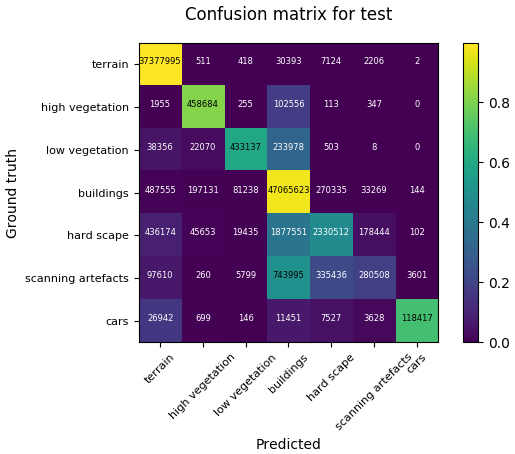
\includegraphics[width=8cm]{fig/test_neighbourhood_classifier.png} }}
    \caption{Matrices de confusion pour le test, avec et sans apprentissage de la relation de voisinage. Avec l'apprentissage de la relation de voisinage, on observe une amélioration des résultats de test pour les classes qui avaient été mises de côté jusqu'ici (\texttt{végétation basse}, \texttt{aménagement urbain}, \texttt{artefact de numérisation} et \texttt{voiture}. Ceci traduit une meilleure capacité à segmenter ces objets, ce qui permet sur le plan de l'apprentissage des classes de mieux se représenter ces objets et au moment de l'inférence de mieux classifier ces objets.}
    \label{fig:neighbourhood}
\end{figure}

% Test set precision metrics with and without neighbourhood classifier
\begin{table}[p]

\caption{Précision (\%) au niveau des composantes connexes et des points, avec et sans apprentissage de la relation de voisinage. Pour les nuages de l'ensemble d'entraînement on remarque un amélioration de la précision lorsque la vérité terrain est donnée au niveau des points. Ceci témoigne directement du fait que la segmentation est meilleure avec l'apprentissage de la relation de voisinage. De même, pour les nuages de test on a globalement de meilleurs résultats lorsque la relation de voisinage est apprise.}


\begin{tabular}{l|c|c|c|c|}
\cline{2-5} & \multicolumn{4}{c|}{données d'entraînement} \\
\cline{2-5} & \multicolumn{2}{c|}{domfountain1} & \multicolumn{2}{c|}{untermaederbrunnen1} \\
\cline{2-5} & comp. & point & comp. & point \\
\hline
\multicolumn{1}{|l|}{critère de voisinage} & \textbf{100} & 92 & \textbf{100} & 93 \\
\hline
\multicolumn{1}{|l|}{apprentissage supervisé} & 99 & \textbf{98} & \textbf{100} & \textbf{96}\\
\hline
\end{tabular}

\bigskip

\begin{tabular}{l|c|c|c|c|c|c|c|c|}
\cline{2-9}
& \multicolumn{8}{|c|}{données de test}\\
\cline{2-9}
& \multicolumn{2}{|c|}{domfountain2} & \multicolumn{2}{c|}{domfountain3} & \multicolumn{2}{c|}{neugasse} & \multicolumn{2}{c|}{untermaederbrunnen3}\\
\cline{2-9}
& comp. & point & comp. & point & comp. & point & comp. & point \\
\hline
\multicolumn{1}{|l|}{critère de voisinage} & 94 & 92 & 95 & 94 & 97 & 91 & 90 & 85\\
\hline
\multicolumn{1}{|l|}{apprentissage supervisé} & \textbf{96} & \textbf{95} & \textbf{96} & \textbf{95} & \textbf{98} & \textbf{92} & \textbf{99} & \textbf{96}\\
\hline


\end{tabular}
\label{table:neighbourhood}
\end{table}

\subsubsection{Influence de la réflectance laser et de la couleur}

Les informations de couleur et de réflectance laser n'étant pas toujours présentes dans les nuages de points disponibles sur internet, il nous a paru important d'évaluer l'influence de l'information de couleur et de réflectance laser sur la performance afin de pouvoir étudier la capacité du modèle à s'exporter sur un grand nombre de données. Nous avons donc comparé notre méthode avec segmentation du sol en amont et apprentissage de la relation de voisinage pour des nuages avec et sans les informations de couleurs et de réflectance laser. Les résultats sont donnés dans la Table \ref{table:laser_color} et la Figure \ref{fig:laser_color}.

Il est étonnant de noter que là où des expérimentation similaires dans \cite{aka_article} menaient à une dégradation très sensible des résultats en l'absence d'information de couleur, nos résultats sont, pour leur part, stables. Ceci est probablement dû à l'utilisation de notre méthode d'apprentissage de la relation de voisinage qui, semble-t-il, repose plus sur l'information géométrique que sur l'information colorimétrique.

On remarquera toutefois que les classes qui font le plus défaut aujourd'hui (\texttt{végétation basse}, \texttt{aménagement urbain} et \texttt{aretefact de numérisation}) correspondent à des objets de couleurs variées et souvent de matériaux divers, pour lesquels on a donc une variance assez grande sur l'information de couleur et d'intensité. Néanmoins, il est probable que sur un jeu de données plus conséquent, l'approche supervisée puisse extraire des tendances pertinentes à partir de l'information de couleur et de réflectance laser, ce qui améliorerait les résultats.

\begin{figure}[p]
    \centering
    \subfloat[avec couleur et réflectance laser]{{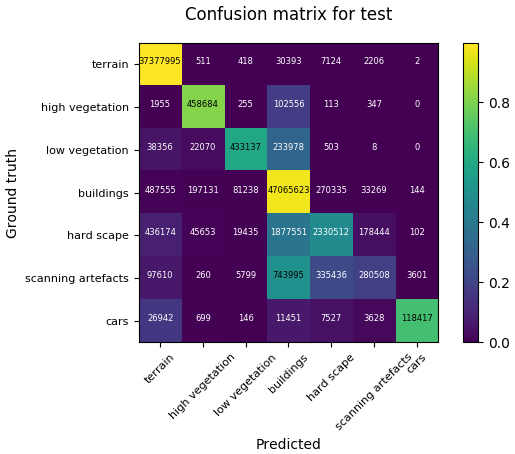
\includegraphics[width=8cm]{fig/test_neighbourhood_classifier.png} }}
    \qquad
    \subfloat[sans couleur ni réflectance laser]{{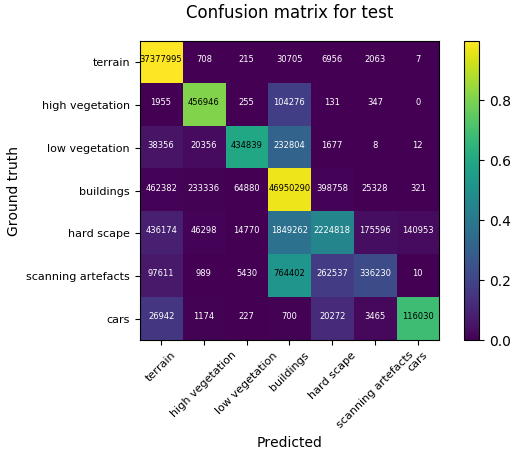
\includegraphics[width=8cm]{fig/test_without_color_nor_intensity.png} }}
    \caption{Matrices de confusion pour le test, avec et sans l'information de couleur et de réflectance laser. Les matrices de confusion sont sensiblement les mêmes. Il semblerait donc que notre méthode d'apprentissage de la relation de voisinage et de la classification des objets ne repose que très peu ou pas du tout sur ce type d'information pour prendre sa décision.}
    \label{fig:laser_color}
\end{figure}

% Test set precision metrics with and without color and intensity information
\begin{table}[p]
\caption{Précision (\%) au niveau des composantes connexes et des points, avec et sans l'information de couleur et de réflectance. Nous obtenons des résultats très similaires dans les deux configurations.}

\begin{tabular}{l|c|c|c|c|}
\cline{2-5}
 & \multicolumn{4}{c|}{données d'entraînement} \\
\cline{2-5} 
 & \multicolumn{2}{c|}{domfountain1} & \multicolumn{2}{c|}{untermaederbrunnen1} \\
\cline{2-5} 
 & comp. & point & comp. & point \\
\hline
\multicolumn{1}{|l|}{avec couleur et reflectance} & 99 & \textbf{98} & \textbf{100} & \textbf{96}\\
\hline
\multicolumn{1}{|l|}{sans couleur ni reflectance} & \textbf{100} & \textbf{98} & \textbf{100} & \textbf{96} \\
\hline
\end{tabular}

\bigskip

\begin{tabular}{l|c|c|c|c|c|c|c|c|}
\cline{2-9}
 & \multicolumn{8}{c|}{données de test}\\
\cline{2-9} 
 & \multicolumn{2}{c|}{domfountain2} & \multicolumn{2}{c|}{domfountain3} & \multicolumn{2}{c|}{neugasse} & \multicolumn{2}{c|}{untermaederbrunnen3} \\
\cline{2-9} 
 & comp.& point & comp. & point & comp. & point & comp. & point \\
\hline
\multicolumn{1}{|l|}{avec couleur et reflectance} & \textbf{96} & \textbf{95} & \textbf{96} & \textbf{95} & \textbf{98} & \textbf{92} & \textbf{99} & \textbf{96}\\
\hline
\multicolumn{1}{|l|}{sans couleur ni reflectance} & \textbf{96} & 94 & \textbf{96} & \textbf{95} & 97 & \textbf{92} & \textbf{99} & 95 \\
\hline
\end{tabular}
\label{table:laser_color}
\end{table}
\subsubsection{Comparaison aux résultats de l'article}

Les résultats présentés ici sont sensiblement moins bons que les résultats de l'article \cite{aka_article} (notamment lorsque l'on compare les matrices de confusion). Là où les auteurs obtiennent un minimum de $80$\% de réussite par classe sur les scènes de test, nous n'avons de résultats tels seulement pour $3$ ou $4$ classes sur $7$ suivant les scènes de test. Plusieurs éléments permettent d'entrevoir pourquoi. Tout d'abord, les classes à identifier dans notre jeu de données (\emph{Semantic3D}) sont plus diversifiées. Nous devons distinguer \texttt{végétation haute} (arbres) et \texttt{végétation basse} (petits buissons) alors que dans l'article qui nous a servi de point de départ, seules les \texttt{arbres} sont à détecter. Autre difficulté, la classe \texttt{aménagement urbain} de notre jeu de données regroupe des objets variés (muret, décoration, panneau de signalisation, panneau publicitaire,  ...) alors que dans l'article, on ne traite que les \texttt{poteaux}. Cette diversité fait que des objets de classes différentes peuvent avoir un certain nombre de caractéristiques communes. Dans ce contexte, la classification est donc plus difficile. Cette plus grande complexité explique aussi pourquoi la relation de voisinage introduite dans \cite{aka_article} et basée le seuillage de quelques paramètres ne marche pas aussi bien que l'apprentissage supervisé de la relation de voisinage sur cette base de données. De plus nous devons traiter des scènes urbaines comme rurales alors qu'elles sont exclusivement urbaines dans l'article. Une difficulté supplémentaire est la non planarité des sols. Enfin, les scènes étudiées ici sont plus étendues que dans \cite{aka_article}. Certains objets éloignés de la source d'acquisition sont peu denses et seulement partiellement visibles, ce qui semble être moins le cas des jeux de données utilisés par les auteurs de l'article.

\subsection{Conclusion}

Lors de ce projet nous avons tenté de reproduire la méthode introduite dans \cite{aka_article}. Nous nous sommes attachés à l'améliorer sur un point qui nous a semblé un peu fragile dans la méthode d'origine : le choix de seuils souvent arbitraires pour segmenter le nuage et classifier les différents objets. Nous nous sommes aperçu, par exemple, que l'application de la méthode telle quelle sur une nouvelle base de données ne donnait pas des résultats optimaux. Nous avons détaillé une méthode robuste pour segmenter le sol. Puis nous avons proposé deux méthodes alternatives pour la segmentation : une méthode de partitionnement spectral et l'apprentissage supervisé de la relation de voisinage. La méthode par partitionnement spectral, si elle a du potentiel, nécessiterait un examen plus approfondi des données ainsi que de la modélisation de l'affinité (la similarité). La méthode par l'apprentissage supervisé a pour sa part immédiatement permis d'améliorer les résultats de segmentation et donc, dans le même temps, de classification. Nous avons également proposé d'utiliser l'apprentissage supervisé pour l'étape de classification. Les résultats ne sont pas encore parfaits mais sont plutôt encourageants. Ils pourraient être largement améliorés avec un entraînement sur une plus grande base de données. Ceci serait même possible dans notre \emph{framework}, puisqu'il permet l'apprentissage simultané sur plusieurs nuages de points.

\clearpage
\newpage

\nocite{*}
\bibliographystyle{plain}
\bibliography{biblio}

\newpage
\appendix
\section{Détail des performances de classification par nuage}
\label{annexe-resultats}

\begin{wrapfigure}{r}{5cm}
\centering
\fbox{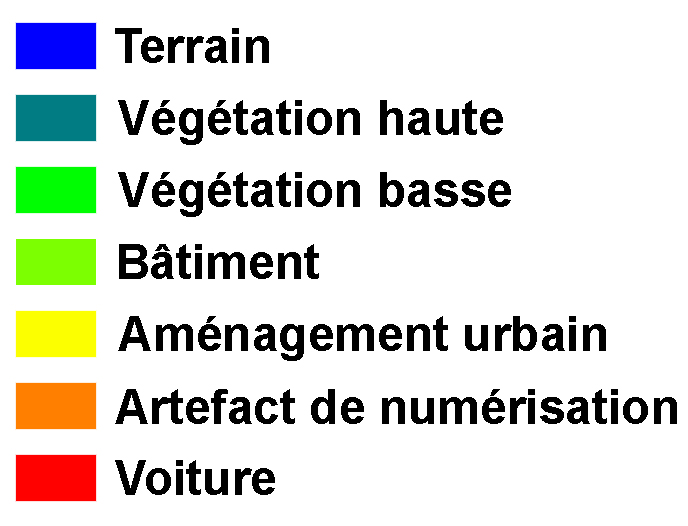
\includegraphics[width=0.2\textwidth]{fig/legend.jpg}}
\end{wrapfigure}

On donne pour chacun des nuages de l'ensemble d'entraînement, de test ou de test supplémentaire (a) la matrice de confusion pour la classification, (b) la segmentation où chaque composante connexe s'est vu attribuer une couleur aléatoire, (c) la prédiction de classification (pour alléger l'affichage, seuls les centres géométriques de chacun des voxels sont représentés), (d) la vérité terrain. La légende pour interpréter les couleurs de la classification sont données ci-contre.

\begin{figure}[h]
    \centering
    \subfloat[matrice de confusion]{{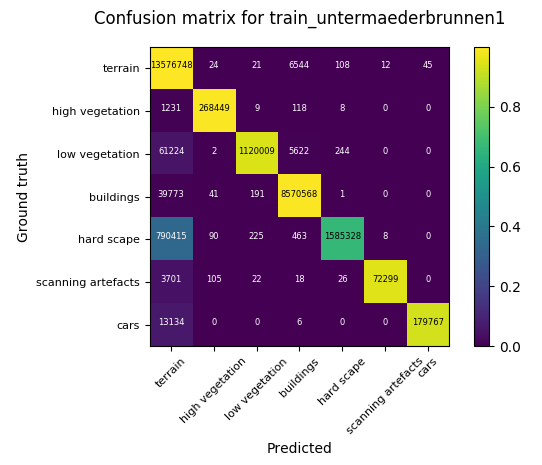
\includegraphics[width=7.6cm]{fig/annexe/train_untermaederbrunnen1.png} }}
    \qquad
    \subfloat[segmentation]{{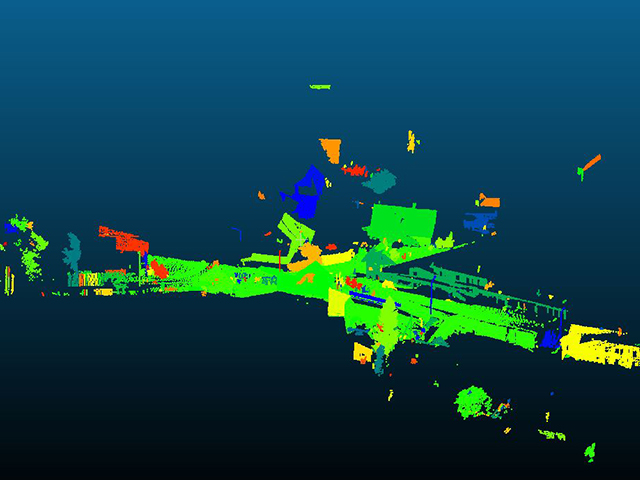
\includegraphics[width=8cm]{fig/annexe/s_untermaederbrunnen1_cc.JPG} }}
    \qquad
    \subfloat[classification]{{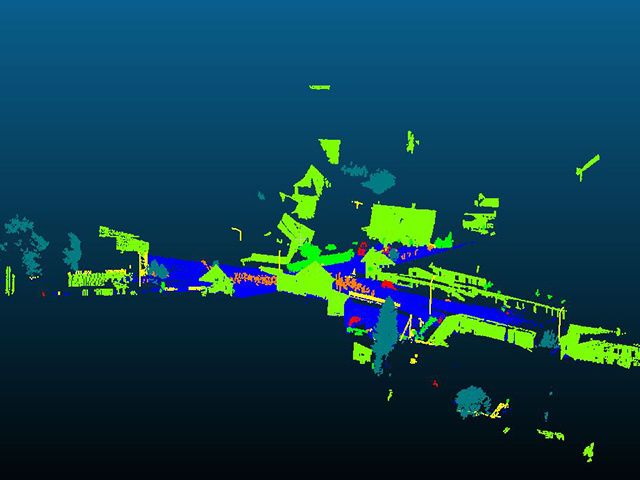
\includegraphics[width=8cm]{fig/annexe/s_untermaederbrunnen1_pc.JPG} }}
    \qquad
    \subfloat[vérité terrain]{{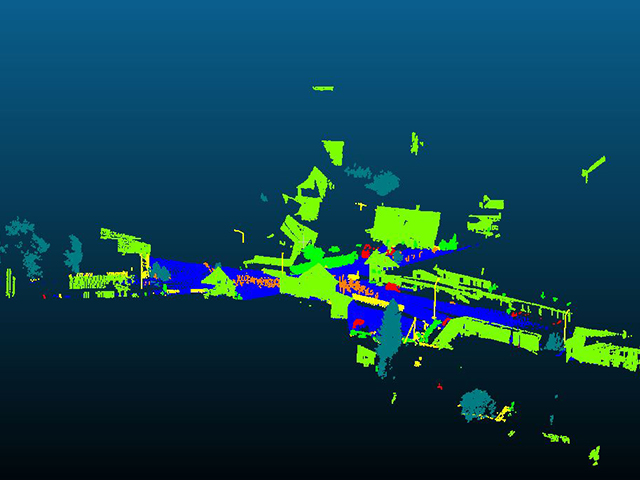
\includegraphics[width=8cm]{fig/annexe/s_untermaederbrunnen1_gt.JPG} }}
    \caption{Nuage d'entraînement : untermaederbrunnen1. Nous obtenons sur ce nuage d'entraînement une très bonne classification. Il est important de rappeler que ceci n'est pas acquis, même pour un nuage d'entraînement car il faut qu'au préalable la segmentation soit bonne. Et il semble, en regardant la figure (b), qu'effectivement la segmentation est satisfaisante.}
    \label{fig:untermaederbrunnen1}
\end{figure}

\begin{figure}[h]
    \centering
    \subfloat[matrice de confusion]{{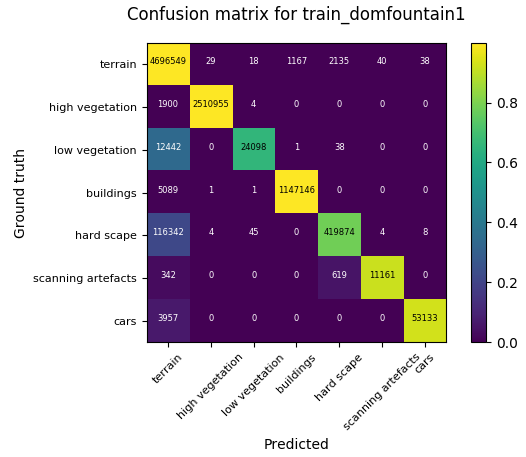
\includegraphics[width=7.6cm]{fig/annexe/train_domfountain1.png} }}
    \qquad
    \subfloat[segmentation]{{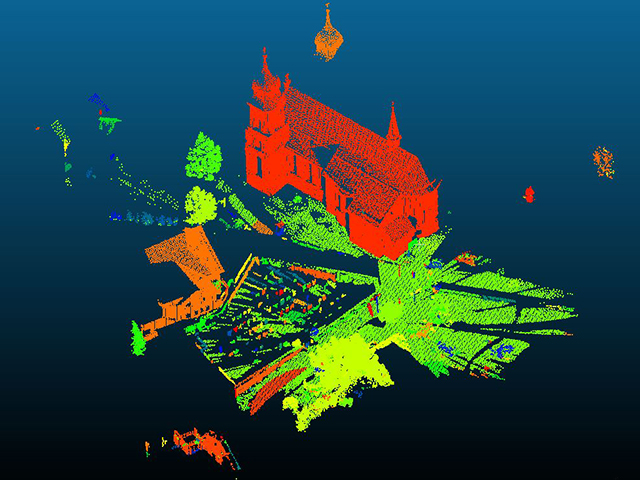
\includegraphics[width=8cm]{fig/annexe/s_domfountain1_cc.JPG} }}
    \qquad
    \subfloat[classification]{{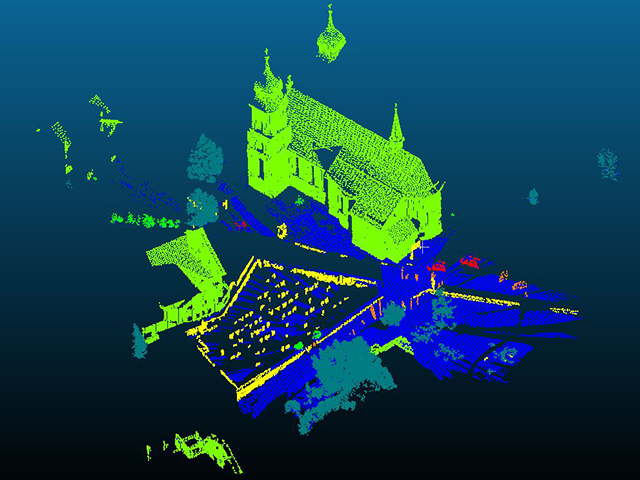
\includegraphics[width=8cm]{fig/annexe/s_domfountain1_pc.JPG} }}
    \qquad
    \subfloat[vérité terrain]{{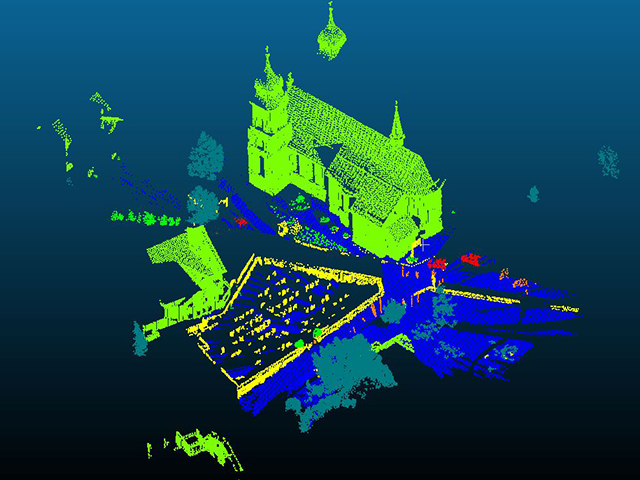
\includegraphics[width=8cm]{fig/annexe/s_domfountain1_gt.JPG} }}
    \caption{Nuage d'entraînement : domfountain1. On fait le même constat que pour le nuage d'entraînement précédent.}
    \label{fig:domfountain1}
\end{figure}

\begin{figure}[h]
    \centering
    \subfloat[matrice de confusion]{{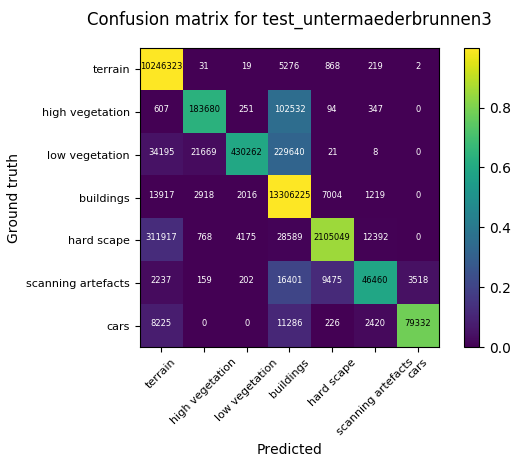
\includegraphics[width=7.6cm]{fig/annexe/test_untermaederbrunnen3.png} }}
    \qquad
    \subfloat[segmentation]{{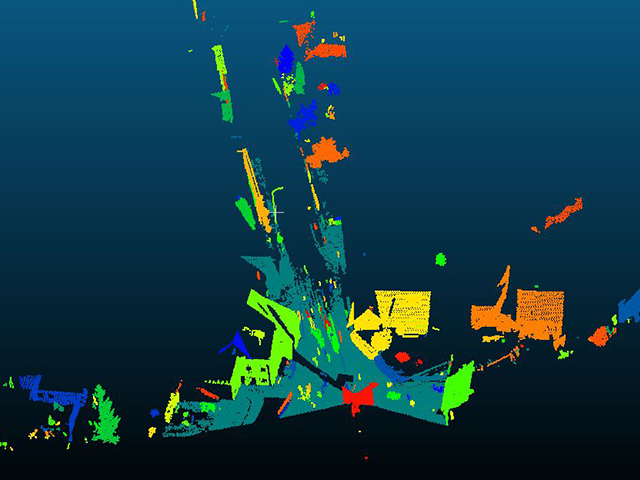
\includegraphics[width=8cm]{fig/annexe/s_untermaederbrunnen3_cc.JPG} }}
    \qquad
    \subfloat[classification]{{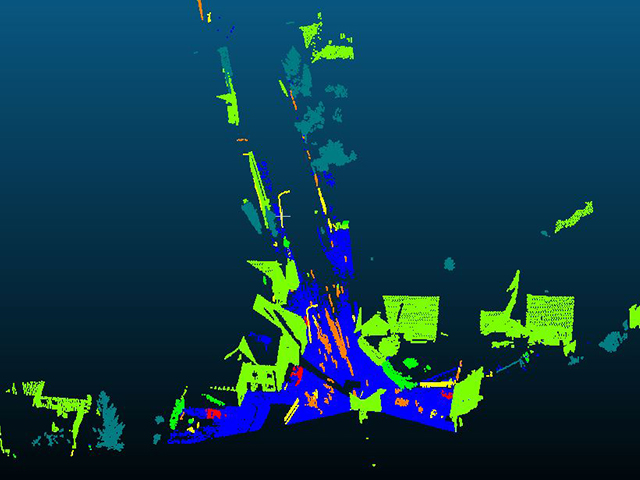
\includegraphics[width=8cm]{fig/annexe/s_untermaederbrunnen3_pc.JPG} }}
    \qquad
    \subfloat[vérité terrain]{{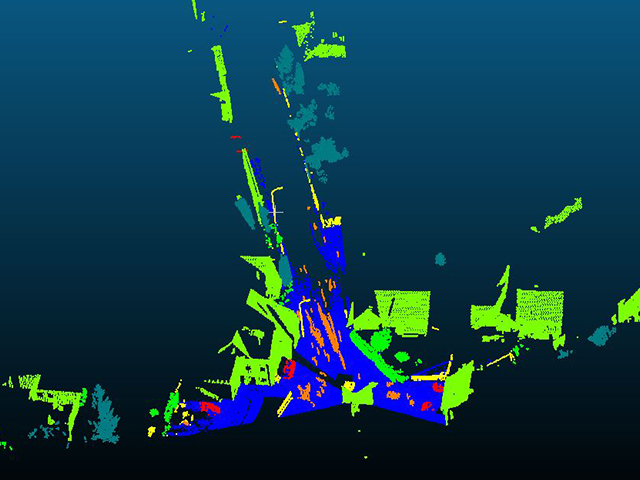
\includegraphics[width=8cm]{fig/annexe/s_untermaederbrunnen3_gt.JPG} }}
    \caption{Nuage de test : untermaederbrunnen3. Les résultats sont concluants pour ce nuage de test, pour chacune des classes une majorité de points a été bien classifiée. La segmentation est dans l'ensemble assez bonne et on note toutefois qu'une faible portion de la \texttt{végétation} a été assimilée à du \texttt{terrain}.}
    \label{fig:untermaederbrunnen3}
\end{figure}

\begin{figure}[h]
    \centering
    \subfloat[matrice de confusion]{{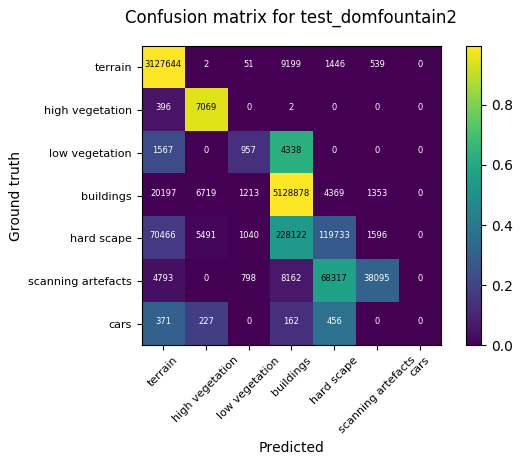
\includegraphics[width=7.6cm]{fig/annexe/test_domfountain2.png} }}
    \qquad
    \subfloat[segmentation]{{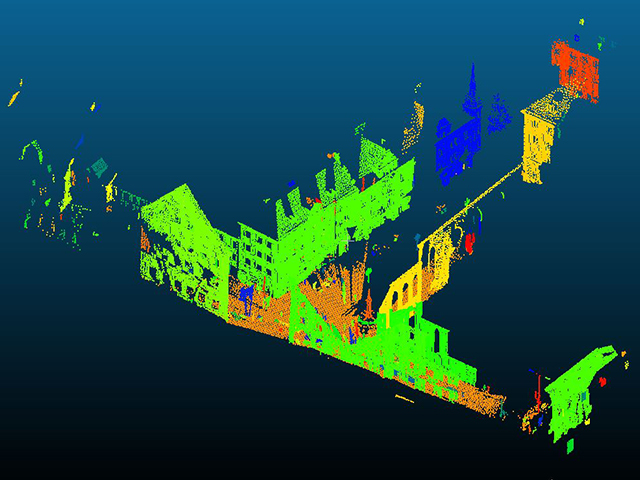
\includegraphics[width=8cm]{fig/annexe/s_domfountain2_cc.JPG} }}
    \qquad
    \subfloat[classification]{{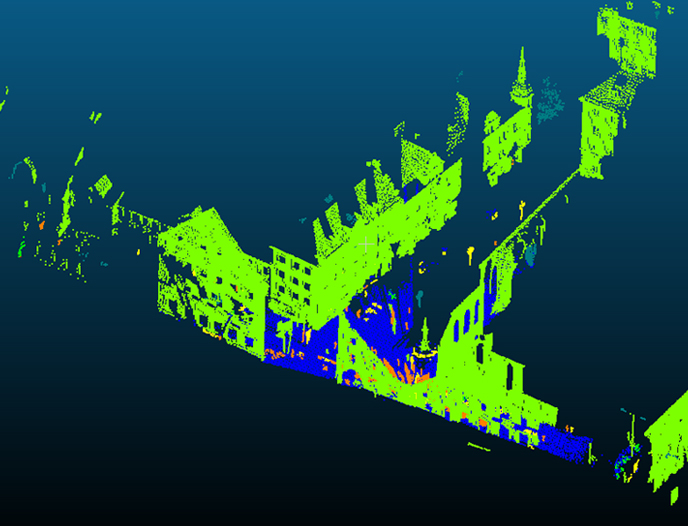
\includegraphics[width=8cm]{fig/annexe/s_domfountain2_pc_2.JPG} }}
    \qquad
    \subfloat[vérité terrain]{{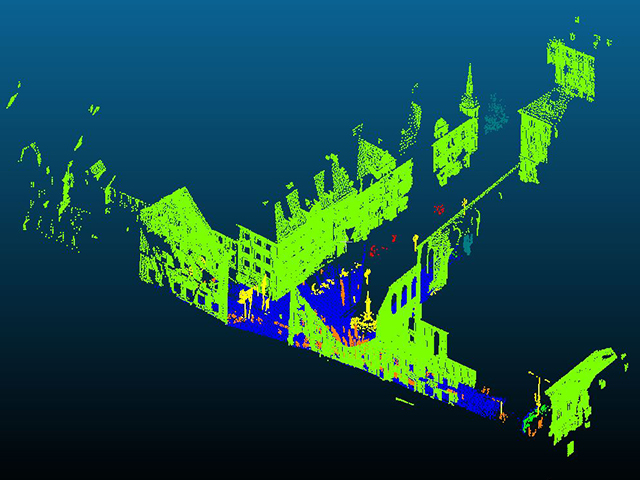
\includegraphics[width=8cm]{fig/annexe/s_domfountain2_gt.JPG} }}
    \caption{Nuage de test : domfountain2. Les résultats sont moins bons sur ce nuage de test. Seules les classes \texttt{terrain}, \texttt{végétation haute} et \texttt{bâtiment} ont bien été classifiées. La \texttt{végétation basse} et les \texttt{aménagements urbains} ont été confondus avec les \texttt{bâtiments}, Les \texttt{artefacts de numérisation} on été pris pour des \texttt{aménagements urbains} et le peu de \texttt{voitures} qu'il y avait n'a pas été détecté en tant que tel. Toutefois la précision globale sur l'ensemble du nuage reste bonne car beaucoup de points appartiennent aux classes \texttt{terrain} et \texttt{bâtiment} qui ont bien été classifiées.}
    \label{fig:domfountain2}
\end{figure}

\begin{figure}[h]
    \centering
    \subfloat[matrice de confusion]{{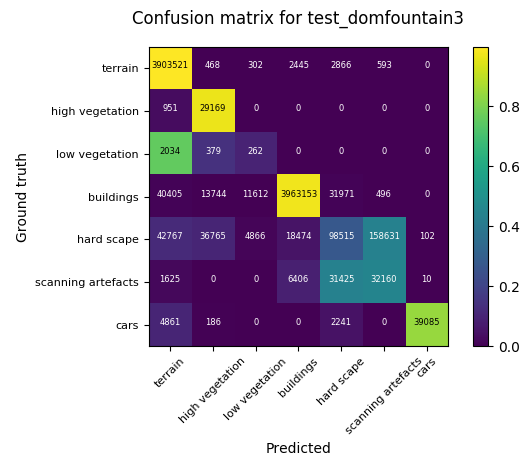
\includegraphics[width=7.6cm]{fig/annexe/test_domfountain3.png} }}
    \qquad
    \subfloat[segmentation]{{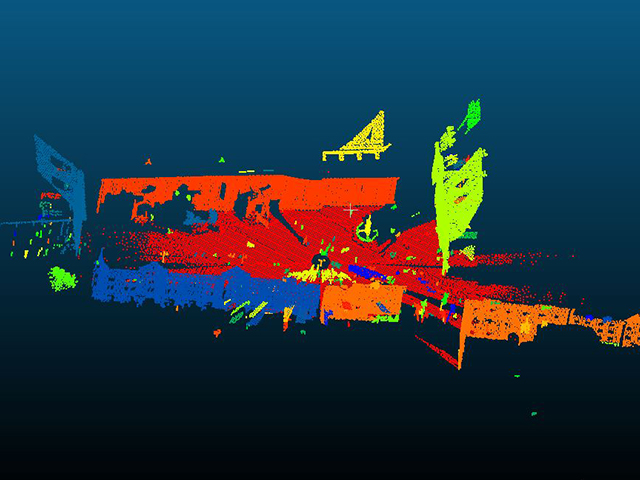
\includegraphics[width=8cm]{fig/annexe/s_domfountain3_cc.JPG} }}
    \qquad
    \subfloat[classification]{{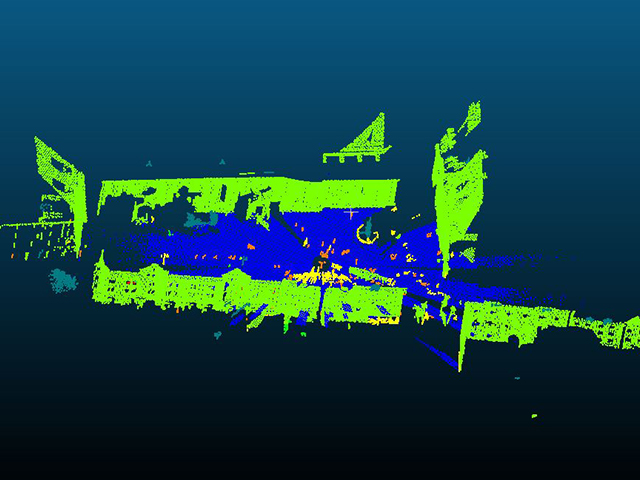
\includegraphics[width=8cm]{fig/annexe/s_domfountain3_pc.JPG} }}
    \qquad
    \subfloat[vérité terrain]{{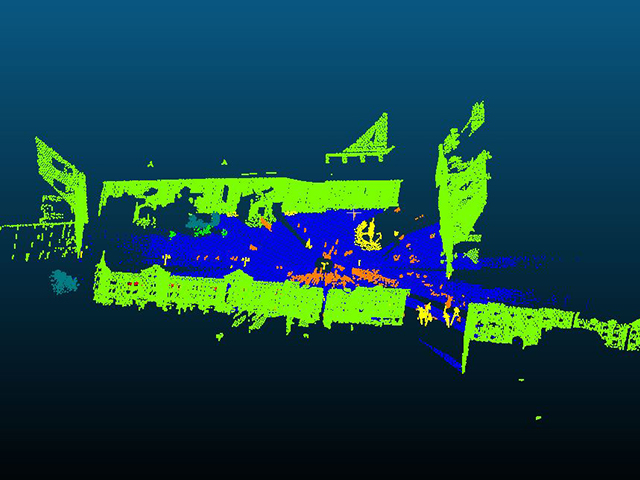
\includegraphics[width=8cm]{fig/annexe/s_domfountain3_gt.JPG} }}
    \caption{Nuage de test : domfountain3. Sur ce nuage de test, plus de la moitié des classes ont été très bien classifiées. Ce n'est pas le cas de la \texttt{végétation basse} mais celle-ci ne correspond qu'à un nombre faible de points. Pour ce qui est des deux classes restantes celles-ci ont été correctement classifiées à hauteur de la moitié des points correspondants.}
    \label{fig:domfountain3}
\end{figure}

\begin{figure}[h]
    \centering
    \subfloat[matrice de confusion]{{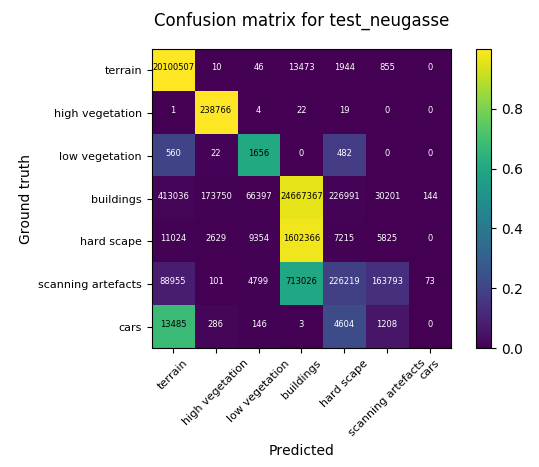
\includegraphics[width=7.6cm]{fig/annexe/test_neugasse.png} }}
    \qquad
    \subfloat[segmentation]{{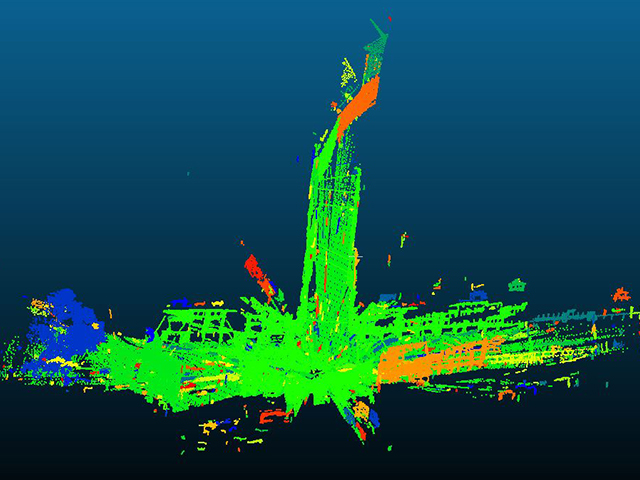
\includegraphics[width=8cm]{fig/annexe/s_neugasse_cc.JPG} }}
    \qquad
    \subfloat[classification]{{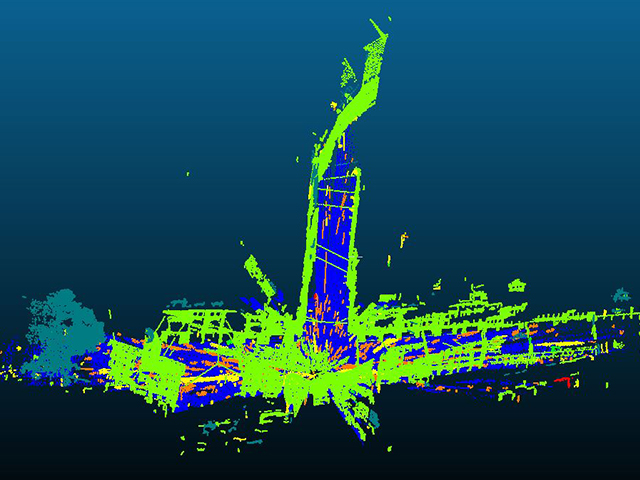
\includegraphics[width=8cm]{fig/annexe/s_neugasse_pc.JPG} }}
    \qquad
    \subfloat[vérité terrain]{{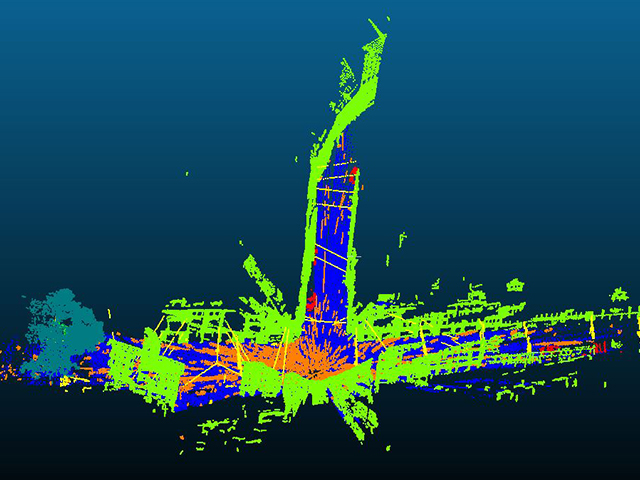
\includegraphics[width=8cm]{fig/annexe/s_neugasse_gt.JPG} }}
    \caption{Nuage de test : neugasse. Un constat à peu près similaire pour ce nuage de test. La classe \texttt{voiture}, peu représentée, n'a pas été très bien classifiée. On remarque un nombre de élevé d'\texttt{artefacts de numérisation}, ce qui ne facilite pas la segmentation du nuage, notamment avec l'assimilation d'une bonne partie de l'\texttt{aménagement urbain} aux \texttt{bâtiments}.}
    \label{fig:neugasse}
\end{figure}

\begin{figure}[h]
    \centering
    \subfloat[matrice de confusion]{{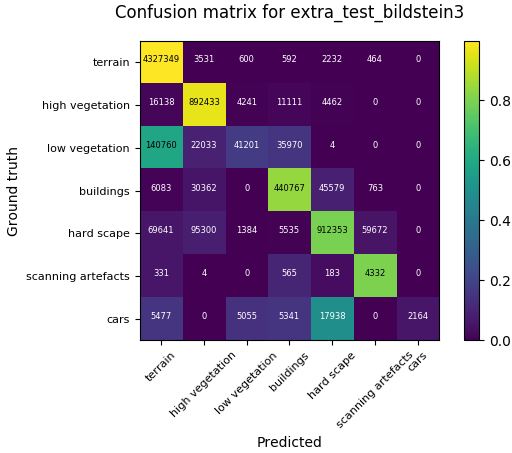
\includegraphics[width=7.6cm]{fig/annexe/extra_test_bildstein3.png} }}
    \qquad
    \subfloat[segmentation]{{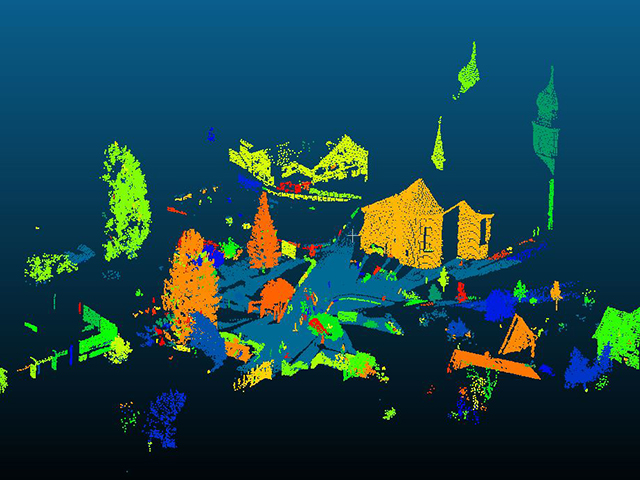
\includegraphics[width=8cm]{fig/annexe/s_bildstein3_cc.JPG} }}
    \qquad
    \subfloat[classification]{{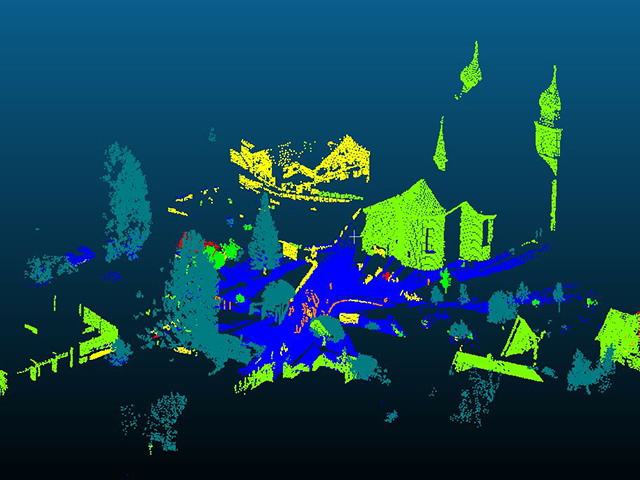
\includegraphics[width=8cm]{fig/annexe/s_bildstein3_pc.JPG} }}
    \qquad
    \subfloat[vérité terrain]{{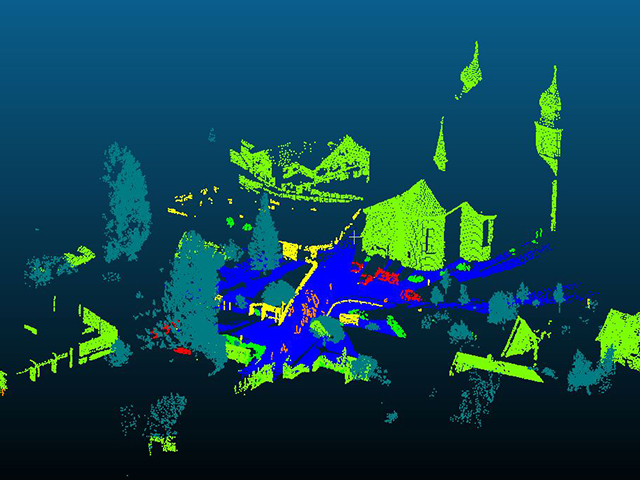
\includegraphics[width=8cm]{fig/annexe/s_bildstein3_gt.JPG} }}
    \caption{Nuage de test supplémentaire : bildstein3. Globalement une assez bonne classification pour ce nuage de test supplémentaire, en dépit des craintes liées à la présence d'une colline dans le nuage de point. Seules les classes \texttt{végétation basse} et \texttt{voiture} ont fait défaut, pourtant plutôt bien segmentées, et on remarque sur l'image que les morceaux de la maison du fond ont été assimilés à de l'aménagement urbain (en jaune), probablement car l'acquisition est peu dense et le toit est absent.}
    \label{fig:bildstein3}
\end{figure}

\begin{figure}[h]
    \centering
    \subfloat[matrice de confusion]{{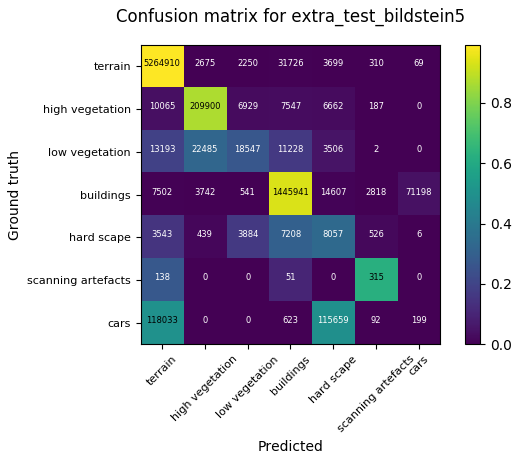
\includegraphics[width=7.6cm]{fig/annexe/extra_test_bildstein5.png} }}
    \qquad
    \subfloat[segmentation]{{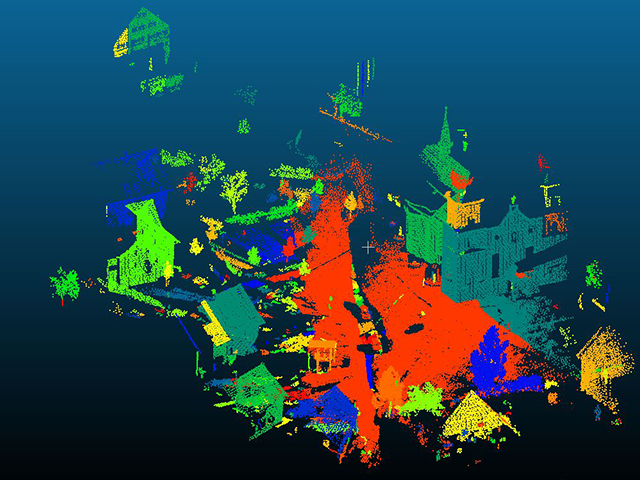
\includegraphics[width=8cm]{fig/annexe/s_bildstein5_cc.JPG} }}
    \qquad
    \subfloat[classification]{{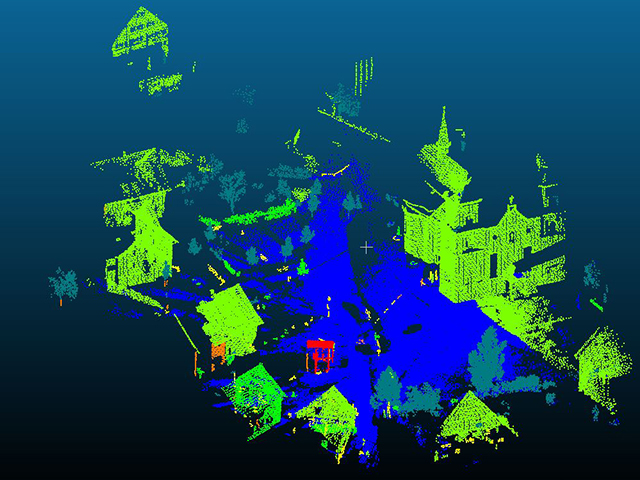
\includegraphics[width=8cm]{fig/annexe/s_bildstein5_pc.JPG} }}
    \qquad
    \subfloat[vérité terrain]{{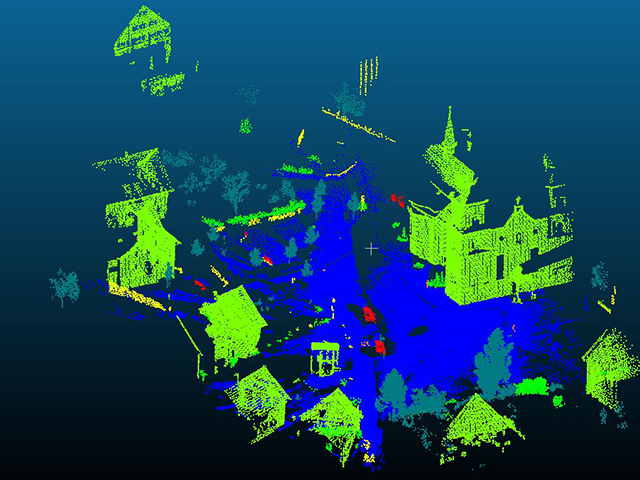
\includegraphics[width=8cm]{fig/annexe/s_bildstein5_gt.JPG} }}
    \caption{Nuage de test supplémentaire : bildstein5. On a, pour ce nuage de test supplémentaire, des résultats acceptables seulement sur les trois classes habituelles (\texttt{terrain}, \texttt{végétation haute} et \texttt{bâtiment}) avec toutefois une partie du terrain segmenté avec l'église à cause de la colline qui n'a permis d'isoler convenablement le sol. Le point le plus problématique est les \texttt{voitures} qui n'ont pas été très bien segmentées. La végétation basse a été confondue entre de multiples classes. Les autres classes ne sont que très peu représentées.}
    \label{fig:bildstein5}
\end{figure}



\end{document}